%%%%%%%%%%%%%%%%%%%%%%%%%%%%%%%%%%%%%%%%%%%%%%%%%%%%%%%%%%%%%%%%%%%%%%%%%%%%%%%%%%%%%%%%%%%%%%%%%%%%%%%%%%%%%%%%%%%%%%%%
\section{La sezione d'urto}\label{sec:sezione-d'urto}
%%%%%%%%%%%%%%%%%%%%%%%%%%%%%%%%%%%%%%%%%%%%%%%%%%%%%%%%%%%%%%%%%%%%%%%%%%%%%%%%%%%%%%%%%%%%%%%%%%%%%%%%%%%%%%%%%%%%%%%%
In quale modo i fisici possono esplorare la struttura di oggetti così
piccoli quali sono gli atomi, i nuclei e le particelle subatomiche?
Quali sono le grandezze fisiche sperimentalmente misurabili e quale tipo
di informazioni su tali oggetti microscopici è effettivamente possibile
ottenere da tali misure?
Gli elementi fondamentali che caratterizzano l'esperimento di
Rutherford(1909-1913) cosí come versioni più moderne sono i seguenti:
\marginnote{L'esperimento di Geiger-Mursden- Rutherford`}

\begin{enumerate}
	\item
	un \textbf{fascio incidente} di particelle proiettile;
	\item
	un \textbf{bersaglio} contenente le particelle da
	studiare(atomi/nuclei /protoni/neutroni);
	\item
	un \textbf{rivelatore} dietro/attorno al bersaglio capace di misurare
	le particelle emergenti\sidenote{Il progresso tecnologico nel campo
	delle macchine acceleratrici ha reso possibile una variante dello
	schema descritto dove la collisione avviene tra le particelle di due
	fasci contrapposti. I `collider', certamente più difficili da
	costruire permettono però di raggiungere, a parità delle tecnologie
	di accelerazione delle particelle, una maggiore energia della
	collisione.}.
\end{enumerate}

Nell'esperimento di Rutherford:

\begin{itemize}
	\tightlist
	\item
	fascio: particelle \(\alpha\) di \(5.6 MeV\)
	\item
	bersaglio: gold foil con spessore di \(8.6 \times 10^{-6}\) cm
	\item
	rivelatore: vetro dipinto da \(ZnS\) scintillante al momento
	dell'incontro con particelle cariche.
\end{itemize}

\textbf{Goal} dell'esperimento: riconoscere le particelle emergenti e
misurarne le grandezze cinematiche(energia, quantità di moto) al fine di
ottenere informazioni sulla natura dell' \textbf{interazione} tra
particella del fascio e particella del bersaglio.

Il termine \textbf{interazione} è un termine generico.
Introduciamo la seguente notazione:

\begin{marginfigure}
	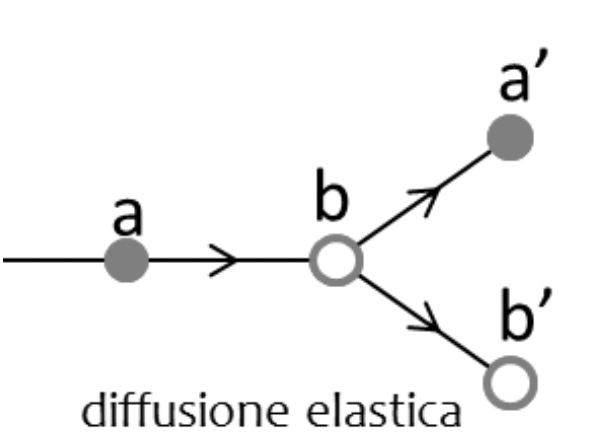
\includegraphics{figs/diffusione-elastica}
	%    \caption{This is a margin figure.}
	\label{fig:diffusione-elastica}
\end{marginfigure}

\begin{itemize}
	\tightlist
	\item
	\textbf{Processi di diffusione}: particelle emergenti dal bersaglio
	coincidono con quelle del raggio incidente
	\item
	\textbf{Processi di produzione}: non vale quanto sopra
\end{itemize}
Tra i processi di diffusione si distinguono processi

\begin{itemize}
	\tightlist
	\item
	\textbf{elastici} : energia della particella incidente \(=\) emergente
	\item
	\textbf{anelastici}: energia della particella incidente \(\neq\)
	emergente
\end{itemize}

Dato che solitamente la particella proiettile è priva di struttura
interna, a differenza di quella bersaglio, si ha diffusione
\begin{marginfigure}
	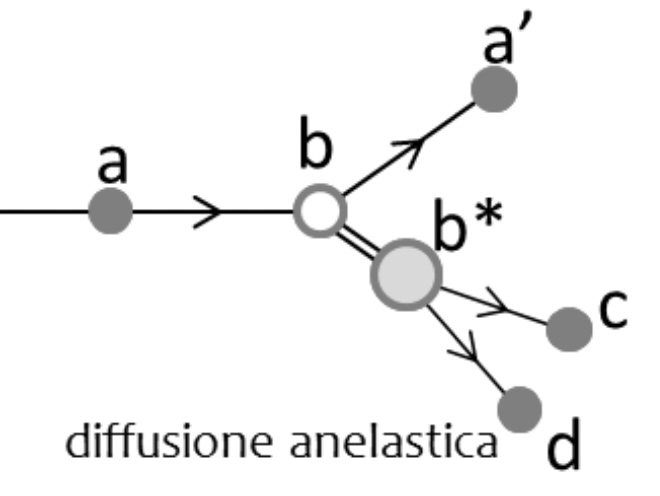
\includegraphics{figs/diffusione-anelastica}
	%    \caption{This is a margin figure.}
	\label{fig:diffusione-anelastica}
\end{marginfigure}

\begin{marginfigure}
	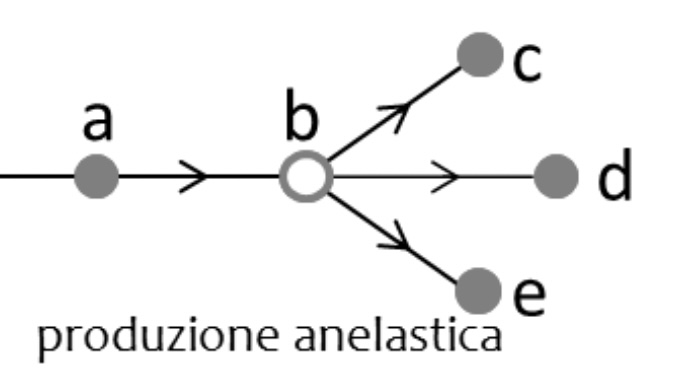
\includegraphics{figs/produzione-anelastica}
	%    \caption{This is a margin figure.}
	\label{fig:produzione-anelastica}
\end{marginfigure}

\begin{itemize}
	\item
	elastica: il bersaglio non modifica la sua struttura e non assorbe
	energia
	\item
	anelastica: il bersaglio modifica la sua struttura e assorbe energia
\end{itemize}

Si parla di \emph{diffusione profondamente inelastica} quando l'energia
della particella proiettile è tale che la De Broglie wavelength
associata risulta molto minore della dimensione della particella
bersaglio \(\rightarrow\) si può definirne la struttura interna(che
varia durante il processo).

Sulla base di questa terminologia è evidente che \textbf{un processo di
produzione è sempre inelastico}.

Vogliamo ora domandarci quale \textbf{grandezza fisica microscopica del
bersaglio} sia possibile misurare con un arrangiamento sperimentale alla
Rutherford.
Per cominciare, occorre tenere presente che nella pratica
sperimentale si cerca di ottenere \textbf{un fascio di particelle
proiettile con densità e velocità uniformi e costanti} da inviare su di
un \textbf{bersaglio materiale chimicamente omogeneo}.
In generale, in
questa situazione, \textbf{si ottengono informazioni sui componenti
microscopici del bersaglio confrontando il fascio di particelle uscente
con quello entrante}.
In particolare maggiore è il numero di grandezze
fisiche del fascio emergente che vengono misurate (distribuzione
spaziale, energia, quantità di moto, tipologia, etc...) più
dettagliata risulterà l'informazione sui componenti microscopici del
bersaglio.

Le assunzioni che faremo sono le seguenti:

\begin{enumerate}
	\tightlist
	\item
	il fascio di sezione trasversale \(\Sigma\) sia costituito da
	corpuscoli massivi puntiformi in moto con la stessa velocità \(v\) e
	densità spaziale \(n_f\) uniforme e costante;
	\item
	il bersaglio sia costituito da sferette massive di raggio dato,
	distribuite con densità \(n_b\)uniforme all'interno di un sottile
	strato materiale di spessore \(\Delta x\) e area maggiore di
	\(\Sigma\)(in modo da utilizzare tutte le particelle del fascio);
	\item
	l'interazione tra particella proiettile e particella bersaglio sia
	assimilabile ad un urto meccanico;
	\item
	a seguito di tale interazione la particella proiettile venga deviata e
	dunque rilevata in una direzione diversa da quella del fascio.
\end{enumerate}
Date queste condizioni, la probabilità che una singola particella
proiettile interagisca con una singola particella del bersaglio vale

\[
	\frac{\sigma}{\Sigma}
\]

dove \(\sigma\) è la sezione trasversale della particella bersaglio e
\(\Sigma\) la sezione trasversale del fascio. Il numero di particelle
deflesse dalla direzione del fascio a seguito dell'urto vale allora

\[
	\Delta N_{def} = \Delta N_f \Delta N_b \frac{\sigma}{\Sigma}
\]dove \(\Delta N_f\) è il numero di particelle del fascio che nel tempo
\(\Delta t\) hanno avuto la possibilità di interagire con le
\(\Delta N_b\) particelle del bersaglio.\\
Ora si noti che le \(\Delta N_f\) particelle del fascio sono contenute
all'interno di un parallelepipedo di area \(\Sigma\) ed altezza
\(v \Delta t\) mentre le \(\Delta N_b\) particelle del bersaglio sono
contenute all'interno di un parallelepipedo di area \(\Sigma\) ed
altezza \(\Delta x\) \textbf{.} Ricordando allora che le densità
volumetriche di particelle del fascio e del bersaglio valgono
rispettivamente \(n_f\) e \(n_b\), si ottengono le seguenti espressioni:

\[
	\Delta N_f = \underbrace{\Sigma v \Delta t}_{ \text{Volume}}n_f
	\qquad
	\Delta N_b = \underbrace{\Sigma  \Delta x}_{ \text{Volume}}n_b
\]

che sostituite forniscono il numero di particelle deflesse nel tempo
\(\Delta t\):

\[
	\Delta N_{def} = \Delta N_f \Delta N_b \frac{\sigma}{\Sigma} =
	(\Sigma v \Delta t \ n_f)(\Sigma \Delta x \ n_b)\frac{\sigma}{\Sigma}
\]

e quindi un rate di deflessione

\[
	\frac{\Delta N_{def}}{\Delta t} = (v n_f)( \Sigma \Delta x n_b) \sigma
\] Invertendo la relazione, otteniamo infine l'espressione della
\textbf{sezione trasversale della particella bersaglio} o
\textbf{sezione d'urto} \begin{equation}
							\boxed{\  \sigma = \frac{1}{(n_fv)(n_b \Sigma \Delta x)}\frac{dN_{def}}{dt} }
\end{equation}

L'interesse di questa espressione risiede nel fatto che mette in
relazione una grandezza fisica microscopica, quale la sezione
trasversale \(\sigma\) della particella bersaglio, con grandezze fisiche
macroscopiche misurabili quali sono i parametri geometrici
\(n_f,n_b,\Sigma,\Delta x\) e \(\frac{\Delta N_{def}}{\Delta t}\).

La grandezza \(\sigma\) è detta \textbf{sezione d'urto totale} o sezione
totale d'interazione ed è ciò che può essere misurato in un tipico
arrangiamento alla Rutherford (questa affermazione va presa cum grano
salis poiché disponendo di un adeguato apparato si possono misurare le
sezioni d'urto in funzione di specifiche variabili d'interesse), ha le
\textbf{dimensioni di un'area} (in questo caso coincidente con l'area
trasversale della particella bersaglio) e dunque si misura in
\(m^2\)(più propriamente in suoi sottomultipli), ed è la grandezza
fisica che \textbf{caratterizza l'interazione tra la generica particella
del fascio e la generica particella del bersaglio}.
Ci attendiamo infine
che tale espressione abbia una \textbf{validità generale} e che possa
essere applicata non solo nel caso specifico dell'urto meccanico da noi
esaminato (impossibile a livello microscopico!) ma anche nel caso più
realistico in cui le particelle del fascio e del bersaglio interagiscono
per mezzo di una interazione naturale.

Infatti, anche nel caso delle particelle subatomiche, nel quale la mutua
interazione non è certo schematizzabile come un urto meccanico di sfere
rigide, sarà sempre possibile introdurre la grandezza microscopica
\(\sigma\) il cui valore, però, non sarà determinato dalla sezione
trasversale della particella ma dalle proprietà della interazione e tra
particella proiettile e particella bersaglio.

Dunque, in fisica nucleare e delle particelle elementari gli esperimenti
su fasci misurano essenzialmente le sezioni d'urto della interazione
elementare fascio-bersaglio.
Quando si dispone di una teoria
quantitativa di tale interazione la grandezza \(\sigma\) può essere
calcolata anche teoricamente ed allora, attraverso il confronto con il
valore determinato sperimentalmente, risulta possibile saggiare la bontà
della teoria stessa.
Nella fisica nucleare e delle particelle elementari
il confronto tra teoria ed esperimento avviene quasi sempre attraverso
le sezioni d'urto.

\begin{marginfigure}
	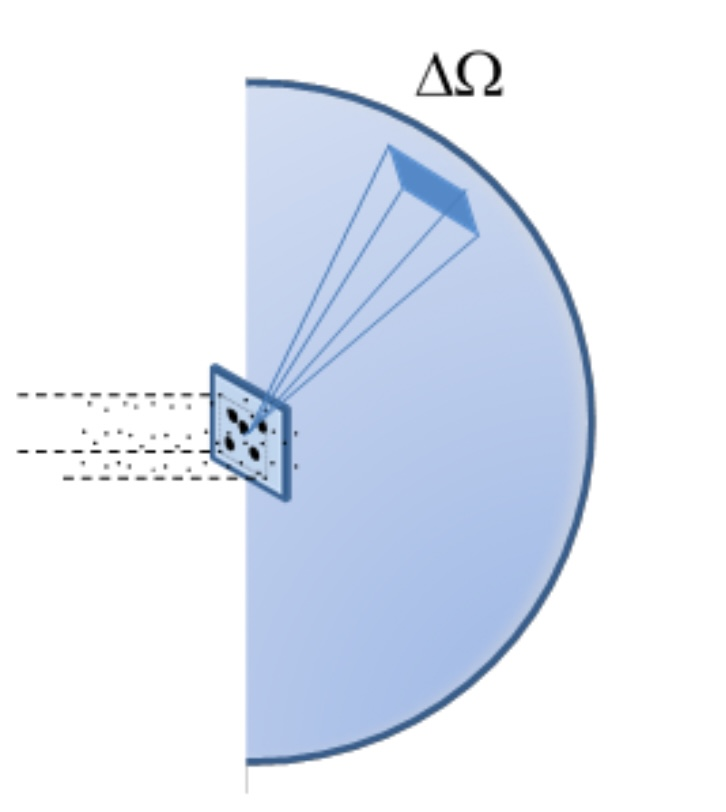
\includegraphics{figs/solid-angle-cross-section}
	%    \caption{This is a margin figure.}
	\label{fig:solid-angle-cross-section}
\end{marginfigure}

Se l'apparato sperimentale è costruito in modo opportuno risulta
possibile andare oltre il semplice conteggio del numero di particelle
deflesse e fornire informazioni sempre più stringenti.
Ad esempio, con
un apparato sperimentale disposto attorno al bersaglio e
\emph{opportunamente segmentato}, in un processo di diffusione risulta
possibile misurare la distribuzione angolare delle particelle del fascio
deflesse dal bersaglio acquisendo ulteriore informazione sperimentale
sulle proprietà della interazione in gioco.
In questo modo si potrà
misurare la sezione d'urto d'interazione con la condizione ulteriore che
la particella proiettile emerga all'interno di un certo angolo solido
elementare \(d \Omega\).
Avremo allora la seguente d'urto elementare
(poiché infinitesimo risulta l'elemento di angolo solido)


\marginnote{Sezione d'urto differenziale \\
	rispetto all'angolo solido}

\[
	d \sigma = \frac{1}{(n_fv)(n_b \Sigma \Delta x)}d \left( \frac{dN_{def}}{dt} \ \text{in} \ d\Omega\right)
\]
in altri termini:
\[
	d \sigma = \frac{1}{(n_fv)(n_b \Sigma \Delta x)} \frac{d\dot{N}_{def \ in \ \Delta \Omega}}{d \Omega} d \Omega
\]

dalla quale otteniamo l'espressione della \textbf{sezione d'urto
differenziale rispetto all'angolo solido} che è la grandezza misurata
dal nostro ipotetico esperimento.
Va da sè che l'integrale di tale
sezione d'urto differenziale rispetto all'angolo solido debba restituire
la sezione d'urto totale

\begin{equation}
	\boxed{ \sigma = \iint_{\Omega}\frac{d \sigma}{d \Omega} \, d \Omega }
\end{equation}

relazione che può essere assunta come definizione della sezione d'urto
differenziale rispetto all'angolo solido.
Se il rivelatore permette di
misurare anche l'energia della particella proiettile sarà possibile
misurare il numero di particelle del fascio che nella unità di tempo
emergono nell'angolo solido elementare \(d \Omega\) all'interno
dell'intervallo elementare \(dE\).
Si ha infatti:
\begin{gather*}
	\frac{d \sigma}{d \Omega} = \frac{1}{(n_fv)(n_b \Sigma \Delta x)}\frac{d}{d \Omega} \left( \frac{dN_{def}}{dt} \ \text{in} \ d\Omega\right)\\
	\frac{d^2 \sigma}{dE d \Omega} = \frac{1}{(n_fv)(n_b \Sigma \Delta x)}\frac{d}{dE}\frac{d}{d \Omega} \left( \frac{dN_{def}}{dt} \ \text{in} \ d\Omega \ \text{e} \ dE\right)\\
\end{gather*}
Il nostro ipotetico esperimento misurerà allora la seguente
\textbf{sezione d'urto doppiamente differenziale in funzione dell'angolo
solido e della energia} definita dalla relazione
\[
	\sigma = \iint_{\Omega}\int_{E} \frac{d^2 \sigma}{dE d \Omega} \, dE \ d \Omega
\]
Gli esempi citati, pur riferendosi a casi particolari chiariscono il fatto, di validità generale, che \emph{il tipo di sezione d'urto misurata dipende essenzialmente dalle caratteristiche tecniche del rivelatore}.

Nel caso più semplice si misurerà una sezione d'urto totale di interazione ma, disponendo di rivelatori via via più sofisticati, risulterà possibile misurare sezioni d'urto differenziali di interazione in funzione di un insieme di variabili cinematiche sempre più ampio.

%%%%%%%%%%%%%%%%%%%%%%%%%%%%%%%%%%%%%%%%%%%%%%%%%%%%%%%%%%%%%%%%%%%%%%%%%%%%%%%%%%%%%%%%%%%%%%%%%%%%%%%%%%%%%%%%%%%%%%%%
\section{Calcoli di sezioni d'urto}\label{sec:calcoli-di-sezioni-d'urto}
%%%%%%%%%%%%%%%%%%%%%%%%%%%%%%%%%%%%%%%%%%%%%%%%%%%%%%%%%%%%%%%%%%%%%%%%%%%%%%%%%%%%%%%%%%%%%%%%%%%%%%%%%%%%%%%%%%%%%%%%
Vediamo due esempi di calcolo di sezioni d'urto :
\begin{description}
	\item[i.] Sezione d'urto differenziale rispetto all'angolo solido di un fascio di proiettili di sezione trascurabile su sfere di raggio $R$ nella ipotesi che abbiano luogo urti classici elastici;
	\item[ii.] Sezione d'urto differenziale di Rutherford.
\end{description}

\smallcaps{ Caso \emph{i}}. \\

Senza entrare nel dettaglio della meccanica dell'urto - assumendo un sistema di coordinate sferiche con asse z lungo l'asse centrale della sfera - sappiamo che sussiste una piena simmetria rispetto all'angolo e l'\textbf{angolo di emergenza} del proiettile è interamente determinato dal \textbf{parametro d'urto} $b$ attarverso una relazione del tipo
\begin{equation}
	b = b(\vartheta)
\end{equation} che codifica i dettagli dell'urto stesso.
\begin{marginfigure}
	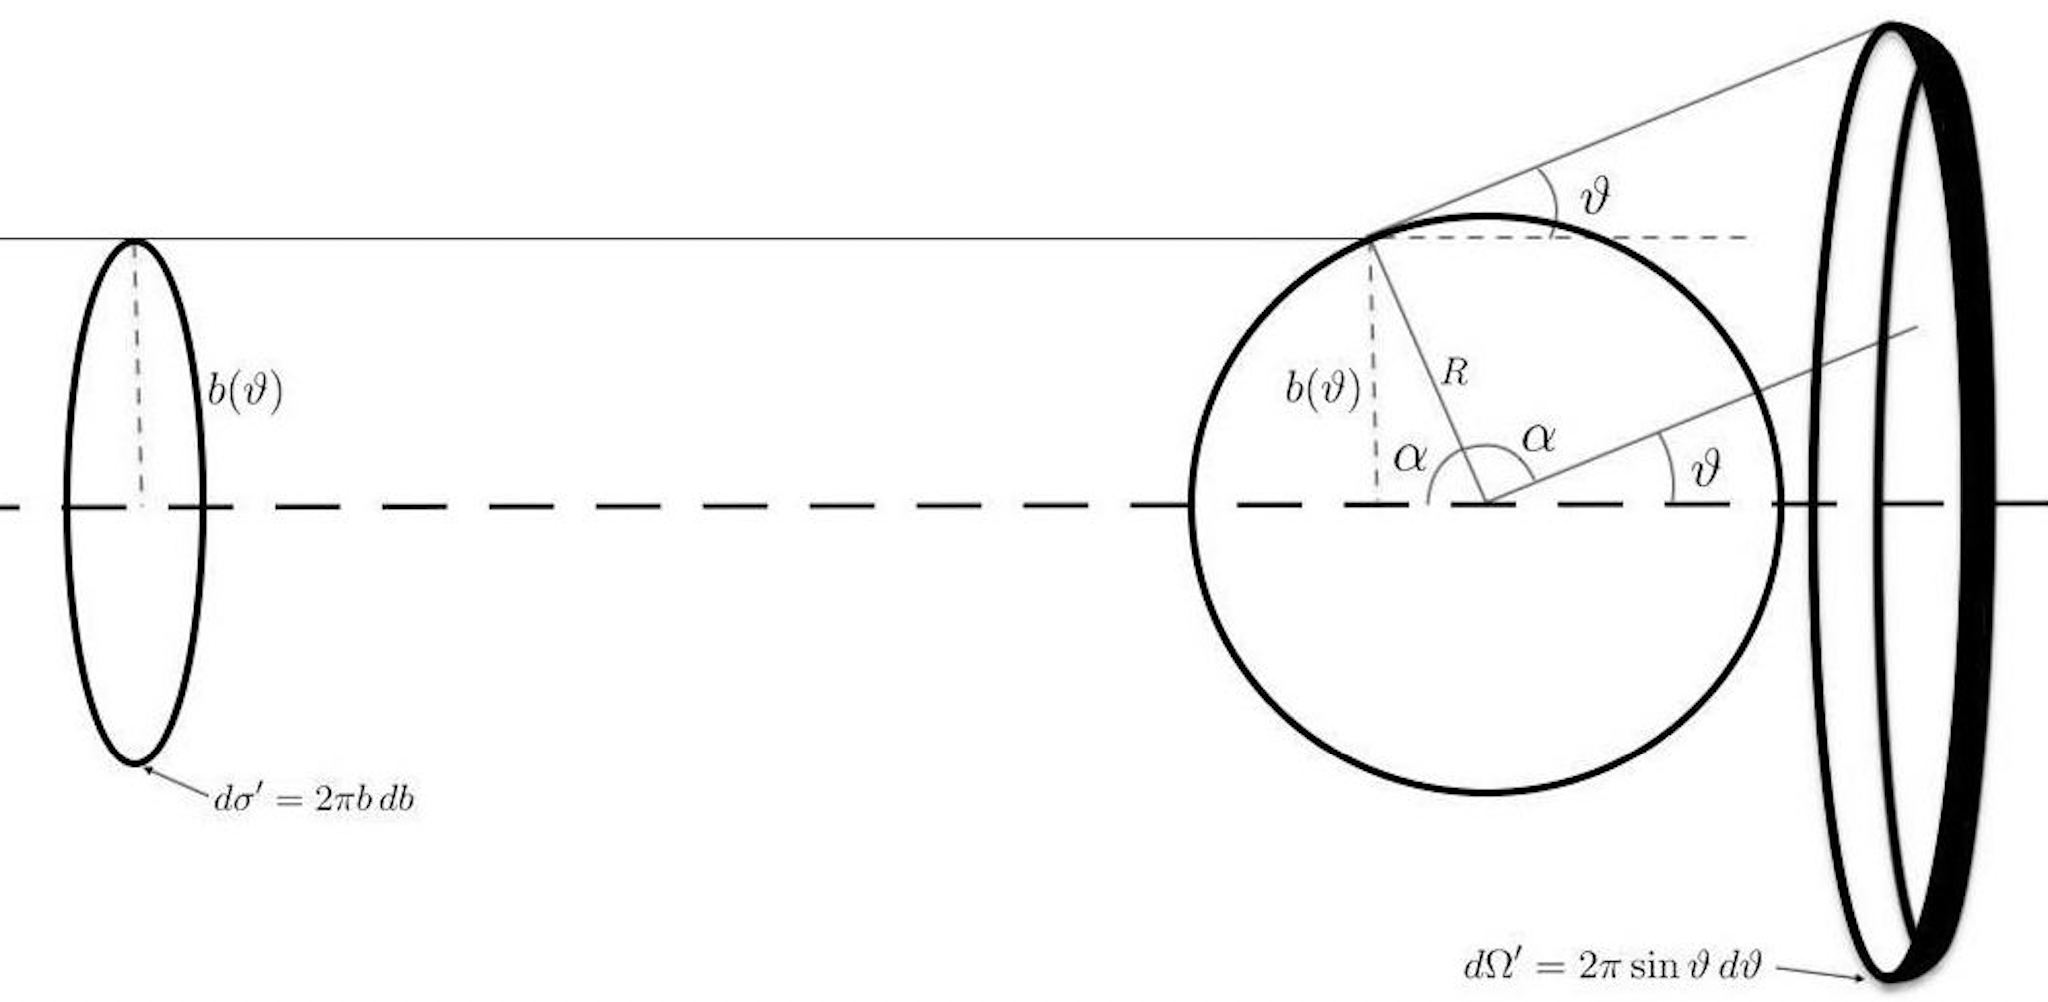
\includegraphics[width = 1.3 \textwidth,scale = 1]{figs/ex-cross-section}
	%    \caption{Sezione d'urto differenziale di una sfera rigida.}
	\label{fig:ex-cross-section}
\end{marginfigure}
Ciò significa che tutti i proiettili passanti per l'area elementare $bd \varphi db$ saranno deflessi dello stesso angolo solido elementare $d \Omega$ per cui, sulla base di ($2$), possiamo scrivere \[
	d \sigma = \frac{d \sigma}{d \Omega}d \Omega = b d \varphi db
\] da cui segue \[
	\frac{d \sigma }{d \Omega} \sin \vartheta d \varphi d \vartheta   =  b d \varphi \left |\frac{db}{d \vartheta}\right | d \vartheta
\] e dunque, infine, la sezione d'urto differenziale rispetto all'angolo solido \begin{equation}
	\frac{d \sigma}{d \Omega} = \frac{b}{sin \vartheta}\left |\frac{db}{d \vartheta}\right |
\end{equation} valida classicamente non solo nel caso della sfera rigida ma in generale.
Per calcolare la sezione d'urto differenziale rispetto all'angolo solido nel caso della sfera rigida di raggio R dobbiamo precisare la forma della ($3$).
Si trova facilmente \[
	\frac{b}{R} = \sin{\alpha}  \qquad \vartheta = \pi - 2 \alpha
\] da cui \[
	b = R \cos{\frac{\vartheta}{2}}
\] Sostituendo nella ($4$) otteniamo \[
	\frac{d \sigma}{d \Omega} = \frac{R \cos{\frac{\vartheta}{2}}}{\sin \vartheta} \left | \frac{d}{d \vartheta}R \cos{\frac{\vartheta}{2}} \right | = \frac{R \cos{\frac{\vartheta}{2}}}{\sin \vartheta}\frac{R}{2} \sin \frac{\vartheta}{2}
\] da cui, infine, la sezione d'urto differenziale della sfera rigida di raggio $R$ \begin{equation}
	\frac{d \sigma}{d \Omega} = \frac{R^2}{4}
\end{equation}

E' immediato verificare che da questa espressione si ottiene una sezione d'urto totale $\sigma = \pi R^2$.

\marginnote{Sezione d'urto differenziale di una sfera rigida}

La formula ($3.4$) può essere utilizzata anche nel caso in cui l'interazione tra le particelle del fascio e quelle del bersaglio non consista in un urto meccanico ma in una interazione mediata da una forza naturale.

\smallcaps{Caso} \emph{ii}. \\

Trattiamo allora il caso della \textbf{diffusione di Rutherford} di proiettili di carica elettrica positiva $ze$ su bersagli di carica elettrica positiva $Ze$ governata dalla forza \[
	\bm{F} = \frac{zZe^2}{4 \pi \epsilon_0}\frac{1}{r^2}\bm{i_r}
\] Come noto tale forza \textbf{conserva il momento angolare} del proiettile \begin{gather*}
	\bm{r} \wedge \bm{F} = \frac{d}{dt}\bm{l} \qquad r \bm{i_r} \wedge \frac{zZe^2}{4 \pi \epsilon_0}\frac{1}{r^2}\bm{i_r} = \bm{0} \quad \bm{0} = \frac{d}{dt}\bm{l} \quad \bm{l}=\bm{K}\\
	\bm{l}_{t = - \infty} = \bm{l}_t \quad (-x \bm{i} + y \bm{j})\wedge(m \dot{x}\bm{i} + m\dot{y}\bm{j})_{t = - \infty} = r \bm{i_r} \wedge m(\dot{r}\bm{i_r} + r \dot{\varphi}\bm{i_{\varphi}}) \quad - \dot{x}y = r^2 \dot{\varphi}\\
	\dot{x}_{t = - \infty} = v_0 \quad \dot{y}_{t = - \infty} = 0 \quad y_{t = - \infty}= b\\
\end{gather*} da cui
\begin{equation}
	\dot{\varphi} = - \frac{v_0 \ b}{r^2}
\end{equation}
e conserva l'energia del proiettile
\begin{gather*}
	\bm{F} \cdot \bm{v} = \frac{dT}{dt} \rightarrow - \nabla V \cdot \bm{v} = \frac{dT}{dt}\\
	\frac{d(T + V)}{dt} = 0 \qquad E = T + V = K\\
	T_{t = - \infty}+ V_{t = - \infty} = T_{t = + \infty}+ V_{t = + \infty} \qquad V_{t = \pm \infty} =
	- \frac{zZe^2}{4 \pi \epsilon_0}\frac{1}{r_{t = \pm \infty}} = 0 \quad T_{t = - \infty}=T_{t = + \infty}\\
\end{gather*}
da cui si ha
\begin{equation}
	v_0 = v_{t = + \infty}
\end{equation}
Fatte queste premesse conviene risolvere la sola \textbf{equazione del moto trasversale}:
\begin{gather*}
	F_y = \frac{d}{dt}m v_y \quad \ \frac{zZe^2}{4 \pi \epsilon_0}\frac{1}{r^2}\sin \varphi = \frac{d}{dt}mv_y\\
	mv_{y,t= + \infty} - mv_{y,t = - \infty} = \int_{- \infty}^{+\infty} \frac{zZe^2}{4 \pi \epsilon_0}\frac{1}{r^2}\sin \varphi\,dt\\
	v_{y,t= + \infty} = v_{t= + \infty}\sin \vartheta \qquad v_{y,t = - \infty} = 0 \quad \varphi_{t = +\infty} = \vartheta \quad \varphi_{t = - \infty} = \pi\\
	mv \sin \vartheta = - \int_{- \infty}^{+ \infty} \frac{zZe^2}{4 \pi \epsilon_0}\frac{1}{r^2}\sin \varphi \frac{r^2}{v_0b}\,d \varphi = \frac{zZe^2}{4 \pi \epsilon_0 v_0 b}(\cos \vartheta + 1)\\
\end{gather*}
da cui
\begin{equation}
	b = \frac{zZe^2}{4 \pi \epsilon_0 m v^2_0} \cot \frac{\vartheta}{2}
\end{equation}
Ora possiamo derivare questa espressione
\[
	\left | \frac{db}{d \vartheta}\right | = \frac{1}{2}\frac{zZe^2}{4 \pi \epsilon_0 m v^2_0}\frac{1}{\sin^2{\vartheta/2}}
\]
e sostituirla nella $(3.4)$ assieme alla $(3.7)$ ottenendo
\[
	\frac{d \sigma }{d \Omega} = \left( \frac{zZe^2}{4 \pi \epsilon_0m v^2_0}\right) \cot{\frac{\vartheta}{2}}\frac{1}{2 \sin{\vartheta / 2 \cos (\vartheta /2)}}\frac{1}{2}\left( \frac{zZe^2}{4 \pi \epsilon_0m v^2_0}\right)\frac{1}{\sin^2{\vartheta/2}}
\]
da cui la \textbf{sezione d'urto differenziale di Rutherford}

\begin{equation}
	\frac{d \sigma }{d \Omega} = \frac{1}{4} \left( \frac{zZe^2}{4 \pi \epsilon_0m v^2_0}\right) ^2\frac{1}{\sin^4{\vartheta / 2}}
\end{equation} un risultato valido anche in meccanica quantistica.

	[Esercizio in dispensa pag 38.]

%%%%%%%%%%%%%%%%%%%%%%%%%%%%%%%%%%%%%%%%%%%%%%%%%%%%%%%%%%%%%%%%%%%%%%%%%%%%%%%%%%%%%%%%%%%%%%%%%%%%%%%%%%%%%%%%%%%%%%%%
\section{Le proprietà ondulatorie delle particelle microscopiche}\label{sec:proprieta-ondulatorie-delle-particelle-microscopiche}
%%%%%%%%%%%%%%%%%%%%%%%%%%%%%%%%%%%%%%%%%%%%%%%%%%%%%%%%%%%%%%%%%%%%%%%%%%%%%%%%%%%%%%%%%%%%%%%%%%%%%%%%%%%%%%%%%%%%%%%%

Nel 1913, quando Geiger, Mursden e Rutherford compirono il loro
esperimento, interpretarono le collisioni tra particelle del fascio e
atomi del materiale in termini di urti governati dalle leggi della
meccanica classica.
Non potevano fare altrimenti, tuttavia di li poco
Bohr - sulla base dei lavori di Plank ed Einstein - e poi nella decade
successiva De Broglie, Heisenberg, Schrödinger e Born modificheranno
radicalmente il quadro interpretativo introducendo l'idea che \textbf{le
particelle microscopiche, oltre a possedere proprietà corpuscolari,
	dovevano possedere anche proprietà ondulatorie,} per cui ad esse si
doveva associare una lunghezza d'onda e frequenza (De Broglie) ed una
funzione d'onda (Born), soluzione quest'ultima di una determinata
equazione d'onda (Schrödinger), giungendo così alla formulazione della

D'altra parte, a partire dai lavori di Planck sul corpo nero (1900) e di
Einstein sull'effetto fotoelettrico (1905), venne contemporaneamente
affermandosi l'idea che i campi classici maxwelliani - dotati certamente
di proprietà ondulatorie poiché capaci dei fenomeni della interferenza e
diffrazione -- dovevano essere costituiti da enti microscopici (poi
chiamati quanti del campo) dotati anche di proprietà corpuscolari.
Si affermò così il concetto di \textbf{quanto del campo come ente
microscopico intrinsecamente `ibrido' poiché dotato di proprietà sia
ondulatorie che corpuscolari}.
Dato questo stato di cose, si pose naturalmente la domanda se le particelle microscopiche ed i quanti del campo - entrambi dotati di proprietà sia corpuscolari che ondulatorie - dovessero essere pensati come enti distinti oppure no.

La risposta -- fondamento del moderno punto di vista - fu data dalle
teorie di campo quantizzato (formulate alla fine degli anni '20 da
Dirac, Heisenberg, e Jordan) le quali assumono che \textbf{le particelle
microscopiche osservate negli apparati sperimentali devono essere
identificate con i quanti di specifici campi}, superando in tal modo la
ripartizione degli enti fisici in particelle materiali e campi affermata
dalla fisica classica.
Da ciò consegue che \textbf{il linguaggio
naturale della fisica delle particelle debba essere quello della teoria
dei campi quantizzati} tuttavia, quando le energie in gioco non sono
così elevate da rendere necessaria una descrizione relativistica e
soprattutto da rendere possibili processi di creazione e distruzione di
particelle\textbf{, la descrizione offerta dalla meccanica quantistica
ordinaria risulta appropriata}.

Per questo, alle basse e medie energie possiamo certamente assumere che
la fisica nucleare possa essere ben descritta nell'ambito della
meccanica quantistica mentre questo non è certamente più vero nella
fisica nucleare alle alte energie dove possono aversi collisioni tra
nucleoni ad energie di centinaia o migliaia di GeV per nucleone (Alice
ha operato a 2.76 TeV per coppia di nucleoni) e risulta necessaria una
descrizione dei processi basata sulle teorie di campo quantizzato.

Volendo richiamare in modo diretto ed euristico alcuni concetti di
meccanica quantistica, si può cominciare scrivendo \textbf{le grandezze
cinematiche fondamentali di una generica onda piana sinusoidale,} ovvero
la \textbf{pulsazione} ed il \textbf{vettore d'onda} collegate tra loro
nella \textbf{relazione di dispersione} che caratterizza le proprietà
fisiche del mezzo in cui l'onda stessa si propaga

\[
	\omega = \frac{2 \pi}{T} \quad \bm{k} = \frac{2 \pi}{\lambda}\hat{k} \quad \omega = \omega(\bm{k})
\]
Scriviamo anche \textbf{le grandezze cinematiche fondamentali di un
generico corpuscolo libero} che corrispondono alle espressioni
relativistiche della \textbf{energia} e \textbf{quantità di moto}
collegate dalla \textbf{relazione energia-impulso}
\begin{equation}
	E = \frac{m c^2}{\sqrt{1 - \frac{v^2}{c^2}}} \qquad \bm{p} = \frac{m \bm{v}}{\sqrt{1 - \frac{v^2}{c^2}}} \qquad E^2 = p^2c^2 + m^2c^4
\end{equation}

Sulla base di considerazioni di natura assai generale, Einstein e De
Broglie ipotizzarono che \textbf{le grandezze ondulatorie e corpuscolari
fossero legate dalle seguenti relazioni} (valide sia nella meccanica
quantistica che nella teoria dei campi quantizzati)
\[
	E = \hp \omega \qquad \bm{p} = \hp \bm{k}
\]
per cui dedussero il seguente legame esplicito tra grandezze
ondulatorie e corpuscolari valido per le particelle microscopiche e le
non meglio precisate \textbf{`onde quantomeccaniche'} o \textbf{`onde di
De Broglie'} a loro associate

\marginnote{Equazioni di De Broglie-Einstein}

\begin{equation}
	E = \hp \omega = \frac{m c^2}{\sqrt{1 - \frac{v^2}{c^2}}} \qquad \bm{p} = \hp \bm{k} = \frac{m \bm{v}}{\sqrt{1 - \frac{v^2}{c^2}}} \qquad \omega^2 = k^{2c}^2+ \frac{m^{2c}^4}{\hp^2}
\end{equation}

La relazione dispersione (relazione energia-impulso) indica chiaramente
che le componenti di Fourier delle `onde quantomeccaniche' si propagano
come se il vuoto fosse un \textbf{mezzo dispersivo}.
Se ad una particella materiale si devono associare grandezze ondulatorie
ad essa si dovrà pure associare una fase ed una certa funzione della
fase detta \textbf{funzione d'onda} il cui significato fisico dovrà
essere precisato.
Una data componente di Fourier di tale onda in forma
piana dovrà comunque avere la seguente semplice espressione\footnote{L'utilizzo
della notazione complessa non è casuale. Infatti alle due espressioni
	\[
		\psi_1(\bm{r},t) = \psi_0 e^{i(\bm{k \cdot r}-\omega t)}
	\] \[
		\psi_2(\bm{r},t) = \psi_0 \sin (\bm{k \cdot r}-\omega t)
	\] sono associate a probabilità differenti \[
		| \psi_1^2| = \psi_0^2
	\] \[
		| \psi_2^2| = \psi_0^2 \sin^2(\bm{k \cdot r}-\omega t)
	\] di cui \emph{solo la prima è in accordo con le verifiche sperimentali}.}


\begin{equation}
	\psi(\bm{r},t) = \psi_0 e^{i(\bm{k \cdot r}-\omega t)} = \psi_{0e}^{\frac{i}{\hp}(\bm{p \cdot r}-E t)}
\end{equation}
Come in un qualunque fenomeno ondulatorio, data la
funzione d'onda si pone il problema di stabilire \textbf{l'equazione
d'onda} ovvero l'equazione che ne governa la dinamica.

Trovare l'espressione formale della equazione d'onda in modo diretto per
una data componente di Fourier non è difficile poiché sappiamo che una
volta sostituita la funzione d'onda (\(12\)) essa non deve fare altro
che restituire la relazione energia-impulso (\(10\)) o la relazione di
dispersione (\(11\)).
A questo scopo vale la pena introdurre le seguenti \textbf{operazioni di differenziazione}

\begin{gather*}
	- i \hp \nabla \psi (\bm{r},t) = - i \hp \nabla \psi_{0e}^{\frac{i}{\hp}(\bm{p \cdot r}-E t)} = - i \hp \psi_{0e}^{\frac{i}{\hp}(\bm{p \cdot r}-E t)} \frac{i}{\hp} \bm{p} = \bm{p}\psi(\bm{r},t)\\
	i \hp \frac{\partial}{\partial t} \psi (\bm{r},t) =  i \hp \frac{\partial}{\partial t} \psi_{0e}^{\frac{i}{\hp}(\bm{p \cdot r}-E t)} =  i \hp \psi_{0e}^{\frac{i}{\hp}(\bm{p \cdot r}-E t)} \left( - \frac{i}{\hp} E\right) = E\psi(\bm{r},t)\\
\end{gather*}
Queste espressioni mostrano che gli operatori differenziali, agendo
sulla generica componente di Fourier, ne determinano la
rimoltiplicazione per i valori della quantità di moto ed energia, un
fatto che suggerisce di definirli come \textbf{operatori della quantità
di moto} ed \textbf{energia}:
\begin{itemize}
	\item
	Operatore della \textbf{quantità di moto}
	\[
	   \hat{P} = - i \hp \nabla    \qquad
	\]
	\item
	Operatore \textbf{dell'energia}

	\[
		\hat{E} = i \hp \frac{\partial}{\partial t}
	\]
\end{itemize}

Nel linguaggio degli operatori, le precenti espressioni possono allora
essere rilette affermando che in una data componente di Fourier
dell'onda quantomeccanica \textbf{i valori della quantità di moto e
della energia sono autovalori degli operatori} \(\hat{P}\) ed
\(\hat{E}\) mentre la funzione d'onda è un loro autostato
\[
	\hat{P}\psi(\bm{r},t) = \bm{p}\psi(\bm{r},t) \qquad
	\hat{E}\psi(\bm{r},t) = E\psi(\bm{r},t)
\]
Introdotti gli operatori energia e quantità di moto, possiamo
partire dalla relazione relativistica energia-impulso della particella
libera ed ottenere la sua equazione d'onda.
I passaggi sono i seguenti
\begin{gather*}
	E^2 = p^2c^2 + m^2c^4\\
	E^2\psi(\bm{r},t) = p^2c^2\psi(\bm{r},t)+m^2c^4\psi(\bm{r},t)\\
	\left( i \hp \frac{\partial}{\partial t}\right)\left( i \hp \frac{\partial}{\partial t}\right)\psi(\bm{r},t) = c^2 (-i \hp \nabla)(-i \hp \nabla)\psi(\bm{r},t)+m^2c^4 \psi(\bm{r},t)\\
\end{gather*}
Si noti che \textbf{tale equazione è lineare per cui deve valere non
solo per la data componente di Fourier ma -- in modo del tutto generale
- per una qualunque sovrapposizione di componenti di Fourier e dunque
per una qualsiasi onda}.

Giungiamo così ad individuare \textbf{l'equazione d'onda} cercata detta
\textbf{equazione di Klein-Gordon} valida per le '\textbf{onde
quantomeccaniche' libere scalari} (senza spin, essendo \(\psi\) scalare)
\marginnote{Equazione di Klein-Gordon}

\begin{equation}
	\nabla^2 \psi(\bm{r},t) - \frac{1}{c^2}\frac{\partial^2}{\partial t^2}\psi(\bm{r},t) =
	\frac{m^2c^2}{\hp^2}\psi(\bm{r},t)
\end{equation}

Tale equazione fu trovata per la prima volta da Schrödinger il quale
però non riuscì a fornire una interpretazione fisica consistente della
funzione d'onda.
Si trattava di un problema cruciale che poteva essere
superato solo interpretando la funzione d'onda nel senso della teoria
dei campi quantizzati (affronteremo questo aspetto in maggior dettaglio
nella seconda parte del corso).
Non essendoci allora i presupposti per
un passaggio di tal genere, Schrödinger rinunciò alla equazione d'onda
relativistica e ripiegò sulla \textbf{equazione d'onda classica} la cui
interpretazione sembrava meno problematica.
Tale equazione la si può
ottenere seguendo esattamente lo stesso tipo di procedimento partendo
però dalla espressione \textbf{energia-impulso classica delle particelle libere}

\[
	E = \frac{p^2}{2m}
\]
Compreso questo fatto, possiamo puntare direttamente a costruire
\textbf{l'equazione d'onda non relativistica per le `onde
quantomeccaniche' inpresenza di forze} aggiungendo il loro potenziale
alla espressione precedente
\[
	E = \frac{p^2}{2m} + V(\bm{r})
\]

Nel caso di una generica componente di Fourier otteniamo allora

\begin{gather*}
	E = \frac{p^2}{2m} + V(\bm{r}) \rightarrow E \psi(\bm{r},t) = \frac{p^2}{2m}\psi(\bm{r},t) +
	V(\bm{r},t)\psi(\bm{r},t)\\
	\left( i \hp \frac{\partial}{\partial t} \right)\psi(\bm{r},t) = \frac{1}{2m}(- i \hp \nabla)(- i \hp \nabla)\psi(\bm{r},t) + V(\bm{r})\psi(\bm{r},t)\\
	i \hp \frac{\partial}{\partial t} \psi(\bm{r},t) = - \frac{\hp^2}{2m}\nabla^2\psi(\bm{r},t)+
	V(\bm{r})\psi(\bm{r},t) = \left[ - \frac{\hp^2}{2m}\nabla^2 + V(\bm{r})\right] \psi(\bm{r},t)\\
\end{gather*}

Data la linearità della equazione, concludiamo che l'espressione
ottenuta deve essere valida non solo per la generica componente di
Fourier ma per una qualunque funzione d'onda.
Definendo allora
l'operatore tra parentesi come \textbf{operatore hamiltoniano}
\(\hat{H}\), otteniamo la seguente \textbf{equazione d'onda di
Schrödinger} valida per le \textbf{`onde quantomeccaniche' scalari
	(senza spin) non relativistiche in presenza di forze}
\marginnote{Equazione d'onda di Schroendinger}


\begin{equation}
	i \hp \frac{\partial}{\partial t} \psi(\bm{r},t) = \hat{H}\psi(\bm{r},t) \qquad
	\hat{H} = - \frac{\hp^2}{2m} \nabla^2 + V(\bm{r})
\end{equation}

Tale equazione rese possibile una interpretazione della funzione d'onda
che - pur non essendo di validità generale - permetteva comunque di
descrivere in modo appropriato i fenomeni quantomeccanici in regime non
relativistico ovvero alle basse e medie energie dove non avvengono
processi di creazione e/o distruzione di particelle.
Tale
interpretazione fu proposta da M. Born ed afferma che \textbf{il modulo
quadrato della funzione d'onda nella posizione} \(\bm{r}\) \textbf{ed al
tempo t rappresenta la densità di probabilità di trovare la particella
materiale in quella posizione ed in quell'istante di tempo a seguito di
una misura di posizione.} Questa ipotesi va a costituire uno dei
fondamentali assiomi interpretativi della meccanica quantistica e
comporta che l'espressione
\begin{equation}
	\left | \psi(\bm{r},t)\right |^2 dV
\end{equation}
rappresenti la probabilità di misurare la particella
materiale al tempo \(t\) all'interno del volume \(dV\) centrato nella
posizione \(\bm{r}\).

I fatti appena richiamati chiariscono che \textbf{l'interazione
particella- proiettile/particella-bersaglio non deve essere pensata come
un processo d'urto meccanico ma, piuttosto, come un processo di
diffrazione/rifrazione dell'onda quantomeccanica associata alla
particella proiettile a seguito della sua interazione con
l'ostacolo-bersaglio}.
Dunque essenzialmente un processo di `\textbf{ottica delle onde quantomeccaniche}' dipendente dal tipo di
interazione in gioco.
Se il bersaglio è totalmente riflettente risulterà un processo di
diffrazione simile a quello di un tratto di muro piazzato sul percorso
di un'onda in acqua.
Se il bersaglio è totalmente assorbente risulterà
un processo di diffrazione simile a quello di un tratto di scogliera.
Se
invece il bersaglio opera come un potenziale di forza avremo un processo
di rifrazione assimilabile alle distorsioni dei fronti d'onda
determinate dalle variazioni di profondità del fondale.
Al netto di
questi dettagli è comunque evidente che \textbf{gli esperimenti
fascio-bersaglio con particelle microscopiche devono essere interpretati
in chiave ondulatoria.}

Ad esempio, se vogliamo esplorare la struttura di un nucleo atomico
dovremo essere in grado di risolvere almeno i singoli nucleoni.
Ma
l'interferenza di due onde provenienti da due diversi nucleoni è
apprezzabile solo se i cammini differiscono di una quantità dell'ordine
della lunghezza d'onda.
\begin{marginfigure}
	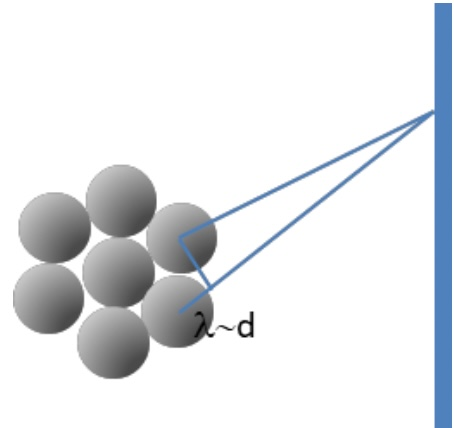
\includegraphics{figs/fascio-bersaglio-de-broglie}
	%    \caption{Sezione d'urto differenziale di una sfera rigida.}
	\label{fig:fascio-bersaglio-de-broglie}
\end{marginfigure}

D'altra parte la differenza di tali cammini è anche dell'ordine delle
dimensioni del singolo nucleone.
Ciò significa che dovremo impiegare
particelle proiettile aventi una lunghezza d'onda di De Broglie
dell'ordine delle dimensioni del singolo nucleone ovvero dell'ordine di
\(1 fm\).
In questo modo saremo sensibili agli effetti
diffrattivi-interferenziali indotti dalla struttura nucleare che potremo
osservare raccogliendo le particelle diffuse su di un rivelatore capace
di misurarne la posizione angolare.
Per quanto riguarda invece la scelta
del proiettile converrà utilizzare i neutroni dato che non risentono
della interazione elettromagnetica che andrebbe a complicare il fenomeno
(si tenga però presente che è più difficile avere a che fare con fasci e
rivelatori di neutroni!).

Ricordando che
\[
	\frac{\hp c}{200 MeV}  \simeq 1 fm
\]
si ha
\begin{gather*}
	p = \hp k = \hp \frac{2 \pi}{\lambda} = \hp \frac{2 \pi}{1} fm^{-1} = \hp 2 \pi \frac{200 MeV}{\hp c}
	\simeq 1.2 \frac{GeV}{c}\\
	\epsilon = \sqrt{p^{2c}^2+m^{2c}^4}\simeq \sqrt{(1.2)^2+(1.0)^2} \simeq 1.5 GeV\\
\end{gather*}
da cui si verifica che con un fascio di particelle di circa $1.2 GeV/c$ di impulso ed $1.5 GeV$ di energia si raggiunge lo scopo.
Se invece vogliamo esplorare la struttura del singolo nucleone dovremo avere un potere risolutivo almeno 100 volte superiore ovvero un impulso $100$ volte maggiore e dunque fasci di particelle di impulso dell'ordine di $100 GeV$.
%%%%%%%%%%%%%%%%%%%%%%%%%%%%%%%%%%%%%%%%%%%%%%%%%%%%%%%%%%%%%%%%%%%%%%%%%%%%%%%%%%%%%%%%%%%%%%%%%%%%%%%%%%%%%%%%%%%%%%%%
\section{Teoria della diffrazione di Kirchoff}\label{sec:teoria-della-diffrazione-di-kirchoff}
%%%%%%%%%%%%%%%%%%%%%%%%%%%%%%%%%%%%%%%%%%%%%%%%%%%%%%%%%%%%%%%%%%%%%%%%%%%%%%%%%%%%%%%%%%%%%%%%%%%%%%%%%%%%%%%%%%%%%%%%

Dato che l'interazione fascio-bersaglio consiste essenzialmente nella
diffrazione delle onde di De Broglie associate alle particelle del
fascio da parte delle particelle del bersaglio, la corretta soluzione
del problema può essere ottenuta cercando l'espressione della funzione
d'onda che:
\begin{enumerate}
	\tightlist
	\item
	soddisfa l'equazione di Schrödinger con potenziale nella regione in
	cui il fascio interagisce con il bersaglio;
	\item
	soddisfa l'equazione d'onda di Schrödinger libera nella regione
	esterna alla interazione prima e dopo il bersaglio;
	\item
	soddisfa la condizione al contorno di essere un'onda piana prima di
	incidere sul bersaglio.
\end{enumerate}
Come noto, la diffrazione delle onde scalari classiche da parte di una
apertura puo' essere trattata in modo rigoroso per mezzo della
\textbf{teoria di Kirchhoff}, dettagliatamente esposta in Appendice
\(1\).
In particolare, se una apertura \(A\) è investita da un'onda
monocromatica, la funzione d'onda diffratta \(\psi(\bm{r})\) in un
generico punto dello spazio \(\bm{r}\) oltre lo schermo è data dalla
seguente espressione:
\begin{marginfigure}
	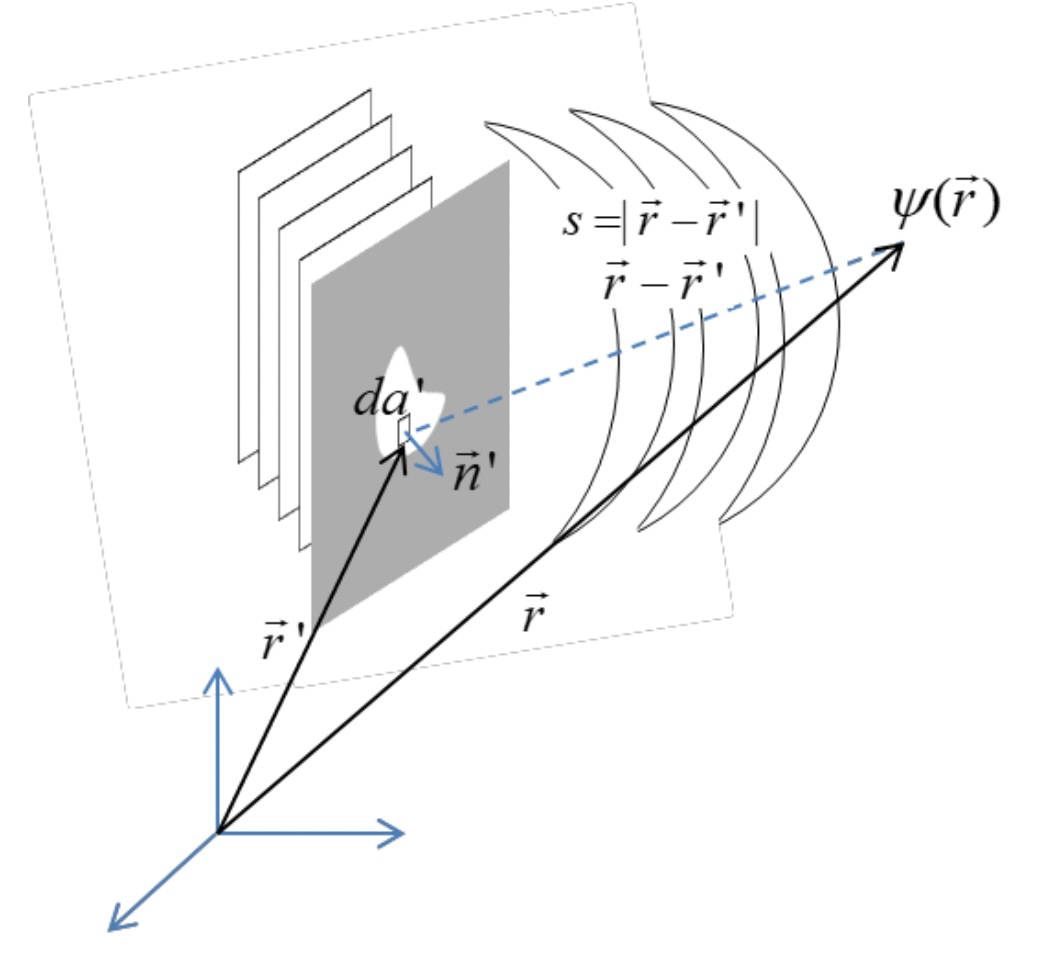
\includegraphics[width = 1.25 \textwidth, height = 1.25 \textheight]{figs/kirchhoff-diffraction-1}
	%    \caption{Sezione d'urto differenziale di una sfera rigida.}
	\label{fig:kirchhoff-1}
\end{marginfigure}

\begin{equation}
	\psi(\bm{r}) = \frac{1}{4 \pi} \iint_{A_p} \left[ \psi(\bm{r'}) (\bm{n}' \cdot \nabla') \frac{e^{iks}}{s} - \frac{e^{iks}}{s}(\bm{n}' \cdot \nabla') \psi(\bm{r}') \right]  \, da'
\end{equation} dove

\begin{itemize}
	\tightlist
	\item \(\bm{r}\) è il vettore posizione del punto di osservazione
	\item \(\bm{r'}\) è il vettore posizione di un punto dell'apertura
	\item \(\psi(\bm{r'})\) è la funzione d'onda calcolata nel punto \(\bm{r'}\)
	dell'apertura
	\item \(\bm{n}'\) è la normale allo schermo nel punto \(\bm{r'}\)
	dell'apertura
	\item \(\nabla'\) è il gradiente della funzione d'onda nel punto \(\bm{r'}\) dell'apertura
	\item \(\bm{k}\) è il modulo del vettore d'onda della funzione d'onda incidente
	\item \(s = | \bm{r} - \bm{r'}|\) è il modulo del vettore congiungente il punto dell'apertura con quello di osservazione
\end{itemize}

Dato che la funzione d'onda \(\psi(\bm{r})\) compare in entrambi i
membri, tale espressione richiede la conoscenza della funzione
\(\psi(\bm{r})\) stessa che si vuole determinare (questo fatto è noto
come `Paradosso di Kirchhoff'). Un circolo vizioso che viene evitato
attraverso\textbf{l'approssimazione di Kirchhoff} la quale assume che la
funzione \(\psi(\bm{r})\) sia non nulla nei soli punti dell'apertura
\(A\) dove coincide conla funzione d'onda monocromatica incidente.
Consideriamo allora il caso di onda piana monocromatica diretta lungo
l'asse delle \(z\) positive incidente su di uno schermo piano normale
all'asse stesso. Si ha
\begin{gather*}
	\psi(\bm{r}) = \psi_0 e^{i \bm{k} \cdot \bm{r}}= \psi_0e^{ik \hat{k}(x \hat{\imath}+y \hat{\jmath}+z \hat{k})}= \psi_{0e}^{ikz}\\
	\bm{n}' = \hat{k}\\
	\psi(\bm{r'}) = \psi_0 e^{i \bm{k} \cdot \bm{r'}}= \psi_0e^{ik \hat{k}(x' \hat{\imath}+y' \hat{\jmath}+z' \hat{k})}= \psi_{0e}^{ikz'}\\
\end{gather*}
e inoltre
\[
	s = \sqrt{(x-x')^2+(y-y')^2+(z-z')^2}
\]
Sviluppiamo ora i termini presenti nell'equazione di Kirchhoff:
\begin{gather*}
	(\bm{n}' \cdot \nabla')\frac{e^{iks}}{s} = \frac{\partial}{\partial z'}\frac{e^{iks}}{s} = ik \frac{e^{iks}}{s}\frac{\partial s}{\partial z'} - \frac{e^{iks}}{s^2}\frac{\partial s}{\partial z'}  = \left( ik \frac{e^{iks}}{s}- \frac{e^{iks}}{s^2} \right)\frac{\partial s}{\partial z'}\\
	(\bm{n}' \cdot \nabla')\psi(\bm{r'}) = \frac{\partial}{\partial z'}\psi_0e^{ikz'}=ik\psi_0e^{ikz'}\\
\end{gather*}
\begin{align*}
	\frac{\partial s}{\partial z'} & = \frac{\partial }{\partial z'}|\bm{r'}-\bm{r}| = \frac{\partial }{\partial z'}\sqrt{(x-x')^2+(y-y')^2+(z-z')^2} \\
	                               & = - \frac{1}{2s}2(z-z') = - \frac{z-z'}{s} = \cos \vartheta
\end{align*}
con $\cos \vartheta = \frac{ (\bm{r'}-\bm{r})\cdot \hat{k}}{|\bm{r'}-\bm{r}|}$.
Da qui ottengo lo sviluppo del primo termine presente nell'equazione di Kirchhoff:
\[
	(\bm{n}' \cdot \nabla')\frac{e^{iks}}{s} = -\left(ik\frac{e^{iks}}{s}-\frac{e^{iks}}{s^2}\right) \cos \vartheta
\]
Sostituendo infine le espressioni di $(\bm{n}' \cdot \nabla ') \frac{e^{iks}}{s}$ e di $(\bm{n}' \cdot \nabla')\psi(\bm{r'})$ in $(16)$ otteniamo
\[
	\psi(\bm{r}) = \frac{1}{4 \pi} \iint_{\text{Foro}} \left[-\psi_0 e^{ikz'}\left( ik\frac{e^{iks}}{s}-\frac{e^{iks}}{s^2}\right) \cos \vartheta - \frac{e^{iks}}{s} ik\psi_0 e^{ikz'} \right] \, da'
\]

\begin{marginfigure}
	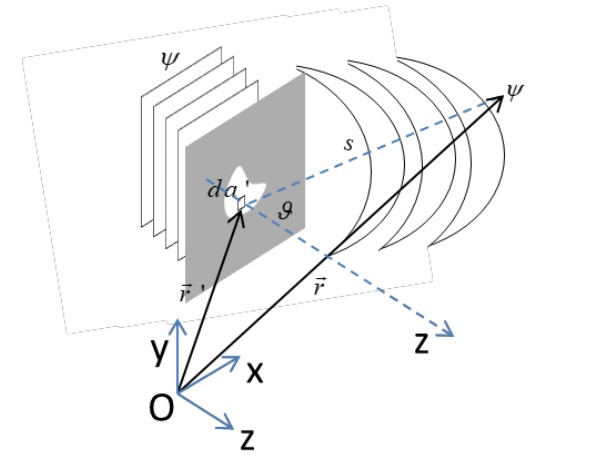
\includegraphics[width = 1.25 \textwidth, height = 1.25 \textheight]{figs/kirchhoff-diffraction-2}
	%    \caption{Sezione d'urto differenziale di una sfera rigida.}
	\label{fig:kirchhoff2}
\end{marginfigure}

Compiamo la seguente \emph{approssimazione}: se il punto di osservazione
è a grande distanza, al primo ordine il termine \(1/s^2\) può essere
trascurato. Abbiamo
\begin{gather*}
	\psi(\bm{r}) \simeq \frac{1}{4 \pi} \iint_{\text{Foro}} \left[-\psi_0 e^{ikz'} ik\frac{e^{iks}}{s} \cos \vartheta - \frac{e^{iks}}{s}ik\psi_0 e^{ikz'} \right]\, da'\\
	\psi(\bm{r}) \simeq -\psi_0 \frac{ik}{4 \pi} \iint_{\text{Foro}} \frac{e^{i(ks+kz')}}{s}(\cos \vartheta + 1)\, da' \simeq -\psi_0 \frac{ik}{2 \pi} \iint_{\text{Foro}} \frac{e^{i(ks+kz')}}{s}\,da'\\
\end{gather*}

\marginnote{$f(\vartheta) = 1 + \cos \vartheta$ fa si che ci sia un fattore che modula l'ampiezza(ad esempio se $\vartheta = 0,f(\vartheta) = 2$ mentre è nullo per $\vartheta = \pi$)}


dove nell'ultimo passaggio si è usato
\(\vartheta << 1 \rightarrow cos \vartheta \simeq 1\). Si noti che
l'espressione integrale ottenuta corrisponde al ben noto principio di
Huygens completato dal \textbf{fattore di obliquità} che modula
l'ampiezza in modo tale da fornire le onde in avanti ed annullare quelle
all'indietro.
Nell'integrale appena ottenuto vogliamo esprimere la fase dell'esponenziale in forma generale attraverso vettori \begin{gather*}
	k(s + z') = k(|\bm{r}-\bm{r'}|+z') = k \left(\sqrt{(\bm{r}-\bm{r'})\cdot(\bm{r}-\bm{r'})}+\bm{n}' \cdot \bm{r'}\right)\\
	= k\left(r \sqrt{1 - \frac{2 \bm{r}\cdot \bm{r'}}{r^2} + \frac{r'^2}{r^2}} + \bm{n}' \cdot \bm{r'}\right) \simeq k\left( r + \frac{r'^2}{2r} - \frac{ \bm{r}\cdot \bm{r'}}{r} + \bm{n}' \cdot \bm{r'}\right)\\
	= k r + k \frac{r'^2}{2r} - k \frac{ \bm{r}\cdot \bm{r'}}{r} + k \bm{n}' \cdot \bm{r'}\\
\end{gather*}
I valori assunti da \(r'\) sono molto minori rispetto a quelli di
\(r\); in particolare se \(D\) è il diametro del foro ed \(L\) la
distanza dallo schermo
\[
	k \frac{r'^2}{2r} \simeq \frac{D^2}{\lambda L}
\]
Se \(\frac{D^2}{\lambda L} << 1\) si parla di \textbf{regime di
Fraunhofer} e il termine in questione può essere trascurato. Si ha
quindi \[
		   k(s+z') \simeq kr - (k \bm{n} - k \bm{n}') \cdot \bm{r}'
\] Introducendo il \textbf{vettore d'onda trasferito}(che parametrizza
lo spostamento del punto di osservazione dall'asse del fascio) \[
																   \bm{q} = k \bm{n} - k \bm{n}'
\] otteniamo infine \[
						k(s+ z') \simeq kr - \bm{q} \cdot \bm{r}'
\] Se il riferimento è interno alla apertura, a seguito della condizione
di Fraunhofer si ha(sistema \(\simeq\) al centro del foro) \[
															   s \simeq r - \bm{n} \cdot \bm{r'} \simeq r - r' \cos \vartheta \simeq r
\]
da cui, si ottiene infine l'espressione cercata della \textbf{funzione
d'onda in campo lontano (o di Fraunhofer) diffratta da una apertura A
investita da un'onda monocromatica}

\begin{equation}
	\psi(\bm{r}) \simeq - \psi_0 \frac{ik}{2 \pi} \frac{e^{ikr}}{r}
	\iint_{ap A} e^{-i \bm{q} \cdot \bm{r}'}\, da'
\end{equation}

Come anticipato però, a noi interessa la situazione complementare,
poiché vogliamo descrivere l'interazione fascio-bersaglio come
diffrazione delle onde di De Broglie del fascio da parte di un ostacolo
avente la forma del bersaglio.

La funzione d'onda \(\psi_{ost A}\) diffratta da uno schermo avente la
forma di A, può essere ottenuta con il semplice \textbf{principio degli
schermi complementari} o \textbf{principio di Babinet.}

La $(17)$ fornisce la funzione d'onda diffratta dalla apertura $A$ come integrale dei contributi degli elementi d'area di $A$.
E' chiaro che la funzione d'onda $\psi_{ost A}$, diffratta da uno schermo avente la stessa forma di A, deve essere data da un integrale dei contributi degli elementi d'area della superficie complementare CA. Ne consegue che la somma delle funzioni d'onda $\psi_{ap A}+ \psi_{ost A}$ debba essere data da un integrale dei contributi degli elementi d'area del piano inifinito contenente $A$, integrale che deve restituire l'onda monocromatica piana incidente \[
	\psi_{ap A}(\bm{r})+ \psi_{ost A}(\bm{r}) = \psi_0e^{i \bm{k} \cdot \bm{r}}
\]
\begin{marginfigure}
	\centering
	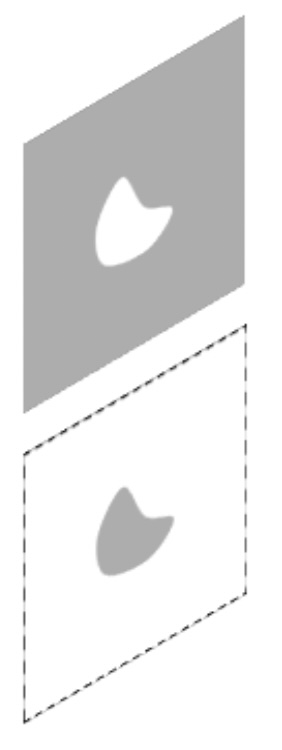
\includegraphics[width = .8 \textwidth, height = .8 \textheight]{figs/kirchhoff-diffraction-3}
	%    \caption{Sezione d'urto differenziale di una sfera rigida.}
	\label{fig:kirchhoff3}
\end{marginfigure}
Da questa relazione possiamo allora ricavare la seguente espressione della \textbf{funzione d'onda diffratta da uno schermo di area A investita da un'onda monocromatica}
\[
	\psi_{ost A}(\bm{r}) =  \psi_0e^{i \bm{k} \cdot \bm{r}}- \psi_{ap \  A}(\bm{r}) \simeq \psi_0e^{i \bm{k} \cdot \bm{r}} + \psi_0 \frac{e^{ikr}}{r} \frac{ik}{2 \pi} \iint_{ost}e^{-i \bm{q} \cdot \bm{r'}} \, da'
\]
All'interno dell'integrale di superficie di questa espressione conviene introdurre la \textbf{funzione di profilo} $\Gamma$(nota anche come \`f̀unzione pupilla" in ottica classica) la quale, nel caso di una apertura A totalmente trasparente, risulta definita nel modo seguente
\[
	\Gamma =
	\begin{cases}
		1   \quad \text{all'interno di } A \\
		0  \quad \text{all'esterno di } A
	\end{cases}
\] Si ha allora \[
	\psi_{ost A}(\bm{r}) \simeq \psi_0e^{i \bm{k} \cdot \bm{r}} + \psi_0 \frac{e^{ikr}}{r} \frac{ik}{2 \pi} \iint_{S_B} \Gamma e^{-i \bm{q} \cdot \bm{r'}} \, da'
\] dove $S_B$(superficie del bersaglio) è il piano infinito contenente lo schermo/ostacolo $A$.

Si noti che ammettendo valori di $\Gamma$ interni ad $A$ inferiori ad $1$, descriviamo un ostacolo A non più totalmente assorbente come uno schermo, ma piuttosto parzialmente trasparente: nel caso limite in cui $\Gamma = 0$ abbiamo infatti un ostacolo $A$ totalmente trasparente che non genera alcuna diffrazione e restituisce l'onda piana incidente.

Potremmo ottenere la massima generalità ammettendo che $\Gamma$ possa dipendere dalla posizione $\bm{r}'$ in $A$ ed assumere anche valori immaginari in modo da descrivere eventuali effetti assorbitivi.
Una simile funzione di profilo ci permette di estendere la diffrazione di un ostacolo $A$ totalmente assorbente al caso generale della diffrazione di un ostacolo $A$ modulante e variamente trasparente, capace di descrivere la diffrazione della fuznione d'onda da parte della materia nucleare.
Sulla base di queste considerazioni, la funzione d'onda assume la forma seguente (lascieremo cadere d'ora in avanti il pedice 'ost')
\[
	\psi_{ost A}(\bm{r}) \simeq \psi_0e^{i \bm{k} \cdot \bm{r}} + \psi_0 \frac{e^{ikr}}{r} \underbrace{\frac{ik}{2 \pi} \iint_{S_B} \Gamma(\bm{r}') e^{-i \bm{q} \cdot \bm{r'}} \, da'}_{f(\bm{q})}
	\qquad 0 \leq \Gamma(\bm{r}') \leq 1
\]
Introducendo \textbf{l'ampiezza di diffusione}, che integra i contributi modulanti e assorbenti degli elementi d'area dell'ostacolo corrispondenti ad un certo vettore d'onda trasferito $\bm{q}$
\[
	f(\bm{q}) = \frac{ik}{2 \pi} \iint_{S_B} \Gamma(\bm{r}')e^{-i \bm{q} \cdot \bm{r}'} \, da'
\]
otteniamo la seguente espressione della \textbf{funzione d'onda in campo lontano diffratta da un ostacolo modulante e assorbente}
\begin{equation}
	\psi_0(\bm{r}) = \psi_0 \left(e^{i \bm{k} \cdot \bm{r}} +
	f(\bm{q}) \frac{e^{ikr}}{r}\right)
\end{equation}

\begin{marginfigure}
	\centering
	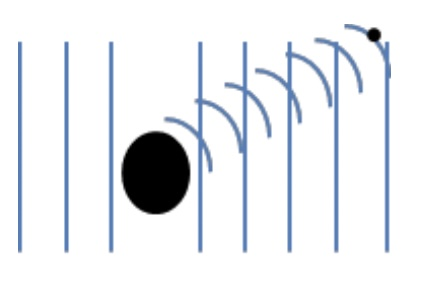
\includegraphics{figs/kirchhoff-diffraction-4}
	%    \caption{Sezione d'urto differenziale di una sfera rigida.}
	\label{fig:kirchhoff4}
\end{marginfigure}

Tale espressione mostra che la figura di diffrazione prodotta da un ostacolo in un dato punto dello spazio è il risultato della interferenza dell'onda piana incidente con l'onda sferica proveniente dall' ostacolo modulata dall'ampiezza di diffusione.
%%%%%%%%%%%%%%%%%%%%%%%%%%%%%%%%%%%%%%%%%%%%%%%%%%%%%%%%%%%%%%%%%%%%%%%%%%%%%%%%%%%%%%%%%%%%%%%%%%%%%%%%%%%%%%%%%%%%%%%%
\section{Le sezioni d'urto in meccanica quantistica}\label{sec:le-sezioni-d'urto-in-meccanica-quantistica}
%%%%%%%%%%%%%%%%%%%%%%%%%%%%%%%%%%%%%%%%%%%%%%%%%%%%%%%%%%%%%%%%%%%%%%%%%%%%%%%%%%%%%%%%%%%%%%%%%%%%%%%%%%%%%%%%%%%%%%%%
Dalla definizione generale sappiamo che il quoziente tra sezione d'urto
del processo e superficie della sezione del fascio deve fornire la
\emph{probabilità del processo} stesso \[
										   \text{Prob}_{\text{int}}  = \frac{\sigma_{diff}}{\Sigma}
\] un fatto che ci permette di affermare che la sezione d'urto del
processo altro non è che la frazione di sezione del fascio che produce
eventi di quel processo.
D'altra parte, nella meccanica quantistica, la
probabilità di un certo processo può essere calcolata mettendo a
quoziente il modulo quadrato della funzione d'onda del processo
integrato sulla superficie di osservazione \(S_O\) con il modulo
quadrato della funzione d'onda incidente integrata sulla sezione del
fascio \(\Sigma\):
\[
	\text{Prob}_{\text{int}}  = \fraclarg{ \iint_{S_O} |\psi_{diff}|^2 \, dS}{\iint_{\Sigma} |\psi_{inc}|^2| \, d \Sigma}
\]
Otteniamo allora la seguente espressione della \textbf{sezione d'urto
integrale del processo}
\begin{equation}
	\sigma_{int} = \Sigma \fraclarg{\iint_{S_0} |\psi_{diff}|^2 \, dS}{\iint_{\Sigma}|\psi_{inc}|^2 \, d \Sigma}
\end{equation} ed anche quella della \textbf{sezione d'urto elementare
del processo}
\begin{equation}
	d \sigma_{int} = \Sigma \fraclarg{|\psi_{diff}|^2 \, dS}{\iint_{\Sigma}|\psi_{inc}|^2 \, d \Sigma}
\end{equation}
dove l'elemento \(dS\) a numeratore si riferisce, come
detto sopra, al generico elemento di superficie di uno schermo lontano
\(S_O\) su cui osserviamo il processo in esame.
\marginnote
{
	\textbf{Significato fisico della probabilita lungo una superficie(da sistemare)}

	Possiamo vedere la probabilita come qualcosa che fluisce lungo la superficie. Come si scrive un flusso di probabilita su una superficie? Sappiamo gia calcolare quanta probabilita fluisce all'interno di un volume La differenza che sussiste e la stessa che c'e tra densita di carica e densita di corrente \[
		\nabla \cdot \bm{J} = - \frac{\partial \rho}{\partial t}
	\] \[
		\iiint \nabla \cdot \bm{J} \,dV =  - \frac{\partial }{\partial t}\iiint \rho \, dV
	\] \[
		\iint_{S(V)} \bm{J}dS = - \frac{\partial }{\partial t}\iiint \rho \, dV  \qquad \bm{j} = \rho \bm{v}
	\] Questa relazione ci dice: la carica dentro il volume varia in una misura che e uguale al suo flusso di superficie--\> non c'e variazione totale, solo flusso da una parte all'altra--\> cio vale perche le equazioni stabiliscono questo equilibrio

	\[
		\bm{J} = |\psi|^2\bm{v}
	\] \[
		\frac{\iint |\psi_1|^2vds}{\iint |\psi_2|^2vds}
	\] v e costante essendo in un processo di diffusione.
}

Nel caso il processo in esame consista nella diffusione da parte dell'ostacolo, risulta possibile calcolare in pochi passaggi la sezione d'urto di diffusione nell'angolo solido elementare.
Infatti, dalla ($18$) si ottengono subito le seguenti espressioni delle funzioni d'onda incidente e diffusa \[
	\psi_{inc} = \psi_o e^{i \bm{k} \cdot \bm{r}} \qquad
	\psi_{diff} = \psi_o f(\bm{q})\frac{e^{ikr}}{r}
\] tenendo poi conto che l'elemento di superficie di un eventuale schermo $S_O$ di forma sferica può essere espresso come segue \[
	dS = r^2 d \Omega
\] sostituendo nella $(20)$ otteniamo \[
	d \sigma_{diff} = \Sigma \fraclarg{|\psi_0|^2|f(\bm{q})|^2\frac{1}{r^2}r^2 d \Omega}{\iint_{\Sigma}|\psi_0|^2 \, d \Sigma}
	= \Sigma \frac{|\psi_0|^2|f(\bm{q})|^2 d \Omega}{|\psi_0|^2 \Sigma}
	= |f(\bm{q})|^2 d \Omega
\]da cui, infine, si derivano le espressioni della \textbf{sezione d'urto di diffusione differenziale e totale rispetto all'angolo solido}

\begin{equation}
	\frac{d \sigma_{diff}}{d \Omega} = |f(\bm{q})|^2 \qquad
	\sigma_{diff} = \iint_{\Omega}|f(\bm{q})|^2 \, d \Omega
\end{equation} Tale espressione chiarisce che la sezione d'urto differenziale di diffusione rispetto all'angolo solido è data dal modulo quadrato della ampiezza di diffusione, dipendente dal vettore d'onda trasferito che parametrizza l'angolo rispetto alla direzione del fascio.

L' espressione ($18$) della funzione d'onda di diffrazione prodotta da un ostacolo ci permette pure il calcolo della sezione d'urto di assorbimento del fascio incidente.
Tale sezione d'urto può essere ottenuta osservando che la probabilità incidente sulla superficie $S_B$ deve essere assorbita dal bersaglio su $S_B$, oppure diffratta e osservata sullo schermo di osservazione $S_O$.
Tenendo presente che la funzione d'onda incidente è non nulla sulla sezione del fascio $\Sigma$, mentre quella di assorbimento è non nulla sul bersaglio, si ottiene la relazione di bilancio:

\begin{gather*}
	\iint_{\Sigma} |\psi_{inc}|^2 \, dS =
	\iint_{S_O} |\psi_{diffr}|^2 \, dS +
	\iint_{bers} |\psi_{ass}|^2 \, d \Sigma\\
	\iint_{\text{bersaglio}} |\psi_{ass}|^2 \, dS =
	\iint_{\Sigma} |\psi_{inc}|^2 \, d\Sigma -
	\iint_{S_O} |\psi_{diffr}|^2 \, dS\\
\end{gather*} Da quest'ultima e dalla ($19$) otteniamo allora la seguente espressione \[
	\sigma_{ass} =\Sigma \, \fraclarg{\iint_{bers} |\psi_{ass}|^2 \, d \Sigma}{\iint_{\Sigma} |\psi_{inc}|^2 \, d \Sigma}
	= \Sigma \, \fraclarg{\iint_{\Sigma} |\psi_{inc}|^2 \, d\Sigma -
		\iint_{S_O} |\psi_{diffr}|^2 \, dS}{\iint_{\Sigma} |\psi_{inc}|^2 \, d \Sigma}
\] Se lo schermo di osservazione è sufficientemente lontano e soddisfa la condizione di Fraunhofer possiamo usare la funzione d'onda diffusa ($18$) con asse z normale allo schermo del bersaglio \begin{align*}
	|\psi_{inc}|^2   & = |\psi_0|^2                                                                                           \\
	|\psi_{diffr}|^2 & = \left | \psi_0 \left( e^{ikz} + f(\bm{q})\frac{e^{ikr}}{r} \right) \right|^2                         \\
	                 & =  |\psi_0|^2 + |\psi_0|^2 \frac{|f(\bm{q})|^2}{r^2} + 2 |\psi_0|^2 \Re f(\bm{q})\frac{e^{ik(r-z)}}{r}
\end{align*} Integrando sullo schermo si ha: \begin{gather*}
	\iint_{S_O} |\psi_0|^2 \, dS + \iint_{S_O}|\psi_0|^2 |f(\bm{q})|^2\, \frac{dS}{r^2} + \iint_{S_O}2 |\psi_0|^2 \Re f(\bm{q})\frac{e^{ik(r-z)}}{r} \, dS\\
	= |\psi_0|^2 \Sigma + |\psi_0|^2 \sigma_{diff} + 2 |\psi_0|^2 \Re \iint_{S_O} f(\bm{q})\frac{e^{ik(r-z)}}{r} \,dS\\
\end{gather*} Il primo termine si è scritto come $|\psi_0|^2 \Sigma$ (e non $|\psi_0|^2 S)$ in quanto nel caso reale abbiamo identità di aree perche il nucleo e piccolissimo rispetto alla sezione del fascio ed inoltre gli angoli di diffusione sono molto piccoli.

Per quanto riguarda la sezione d'urto di assorbimento si ha
\[
	\sigma_{ass} = \Sigma   \fraclarg{|\psi_0|^2 \Sigma - \left[ |\psi_0|^2 \Sigma + |\psi_0|^2 \sigma_{diff} +  2 |\psi_0|^2 \Re \iint_{S_O} f(\bm{q})\frac{e^{ik(r-z)}}{r} \,dS \right]}{|\psi_0|^2 \Sigma}
\] da cui
\begin{equation}
	\sigma_{ass} = - \sigma_{diff} -  2  \Re \iint_{S_O} f(\bm{q})\frac{e^{ik(r-z)}}{r} \,dS
\end{equation}

Per proseguire negli sviluppi è necessario calcolare l'integrale sullo schermo $S_O$.
Assumendo l'origine del riferimento al centro dell'ostacolo e l'asse z normale al piano che lo contiene e dunque normale anche allo schermo lontano, otteniamo per la fase dell'esponenziale

\begin{marginfigure}
	\centering
	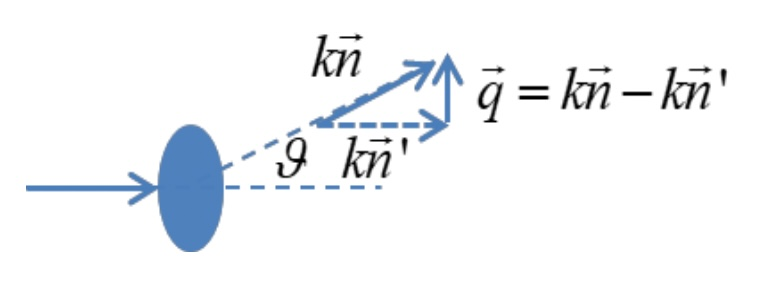
\includegraphics[width = 1.25 \textwidth, height = 1.25 \textheight]{figs/schema-vett-trasferito}
	%    \caption{Sezione d'urto differenziale di una sfera rigida.}
	\label{fig:vett-trasferito}
\end{marginfigure}

\begin{align*}
	r - z & = \sqrt{x^2 + y^2+z^2} -z = z\sqrt{1 + \frac{x^2}{z^2}+\frac{y^2}{z^2}} -z                       \\
	      & \simeq z \left( 1 + \frac{1}{2}\frac{x^2 + y^2}{z^2}\right) -z  = \frac{1}{2}\frac{x^2 + y^2}{z}
\end{align*} Inoltre, se lo schermo è lontano la figura di diffrazione si estende sullo schermo stesso in misura trascurabile, per cui la coordinata z risulta dominare largamente le coordinate x ed y.

Risostituendo nell'integrale che compare nell'espressione di $\sigma_{ass}$ abbiamo \begin{gather*}
	- 2 \Re\iint_{sch}f(\bm{q})\frac{e^{ik(r-z)}}{r} \, dS =
	- 2 \Re f(\bm{o}) \iint_{sch}\frac{e^{ik \frac{x^2 + y^2}{2z}}}{z} \, dxdy\\
	= - \frac{2}{z} \Re f(\bm{o}) \int_{- \infty}^{\infty} e ^{- \frac{k}{2iz}x^2} \, dx
	\int_{- \infty}^{\infty} e ^{- \frac{k}{2iz}y^2} \, dy = - \frac{2}{z} \Re f(\bm{0}) \sqrt{\frac{2iz}{k}}\sqrt{\pi}\sqrt{\frac{2iz}{k}}\sqrt{\pi}\\
	= - \frac{2}{z} \Re f(\bm{0}) \frac{2iz}{k}\pi = - \frac{4 \pi}{k} \Re i (\Re f(\bm{0}) + i  \Im f(\bm{0}))\\
\end{gather*} ottenendo infine \[
	\boxed{\sigma_{diff} + \sigma_{ass} = \frac{4 \pi}{k} \Im f(\bm{0})}
\] risultato noto come \textbf{teorema ottico}.

\marginnote{Teorema ottico}

Questo afferma che la somma delle sezioni d'urto totale di diffusione ed
assorbimento, detta sezione d'urto totale d'interazione, eguaglia (a
meno del fattore moltiplicativo \(\frac{4 \pi}{k}\)) la parte
immaginaria dell'ampiezza di diffusione in avanti (ovvero a vettore
d'onda trasferito nullo).

E' importante sapere che le sezioni d'urto totali di diffusione e
assorbimento possono essere espresse anche attraverso integrali della
funzione di profilo sulla superficie del bersaglio \(S_B\).

Integrando l'ampiezza di diffusione su tutto l'angolo solido nella
(\(21\)) si ottiene la seguente espressione della sezione d'urto totale
di diffusione in funzione del profilo (vedi formula di Kirchhoff in
appendice).
\begin{equation}
	\sigma_{diff} = \iint_{S_B} |\Gamma(\bm{r}')|^2 \, da'
\end{equation}
\begin{gather*}
	\frac{4 \pi}{k} \Im \left(\frac{ik}{2 \pi} \iint \Gamma \, da' \right) =
	\frac{4 \pi}{k} \frac{k}{2 \pi} \Im i \iint(\Re \Gamma +i \Im \Gamma) \, da' =   2 \iint \Re \Gamma \, da'\\
	\iint |\Gamma|^2 \, da' + \sigma_{ass} = 2 \iint \Re \Gamma \, da'\\
	\sigma_{ass} = \iint (2 \Re \Gamma - |\Gamma|^2) \, da'\\
\end{gather*} ma $|1 - \Gamma|^2 = 1 + |\Gamma|^2 - 2 \Re \Gamma$ e dunque si perviene alle espressioni della sezione d'urto totale di assorbimento in funzione del profilo \begin{equation}
	\boxed{ \sigma_{ass} = \iint \left(1 - |1 - \Gamma|^2 \right) \, da' }
\end{equation}
%%%%%%%%%%%%%%%%%%%%%%%%%%%%%%%%%%%%%%%%%%%%%%%%%%%%%%%%%%%%%%%%%%%%%%%%%%%%%%%%%%%%%%%%%%%%%%%%%%%%%%%%%%%%%%%%%%%%%%%%
\section{Diffrazione di un disco assorbente}\label{sec:diffrazione-di-un-disco-assorbente}
%%%%%%%%%%%%%%%%%%%%%%%%%%%%%%%%%%%%%%%%%%%%%%%%%%%%%%%%%%%%%%%%%%%%%%%%%%%%%%%%%%%%%%%%%%%%%%%%%%%%%%%%%%%%%%%%%%%%%%%%

Possiamo usare le formule del precedente paragrafo per calcolare le
sezioni d'urto del processo di \textbf{diffrazione di un'onda piana su
di un ostacolo circolare di raggio R completamente assorbente}.

Adottando un sistema di coordinate polari con l'origine al centro del
disco, la \textbf{funzione di profilo del disco nero} è definita dalle
condizioni
\[
	\Gamma  =
	\begin{cases}
		1  \quad r \leq R \\
		0  \quad r > R
	\end{cases}
\]
Si assuma un riferimento con l'origine al centro del disco e l'asse $z$ normale al piano che lo contiene.
Con questa scelta, se ci limitiamo a considerare angoli di diffusione non troppo grandi, il vettore $\bm{q}$ giace in un piano parallelo a al piano $xy$ e si ha \[
	\bm{q} = \bm{k} ( \bm{n} - \bm{n}') = k ( \sin \vartheta \hat{\imath}_r + \cos \vartheta \hat{k} - \hat{k'}) \simeq
	k \sin \vartheta \hat{\imath}_r
\]

\begin{marginfigure}
	\centering
	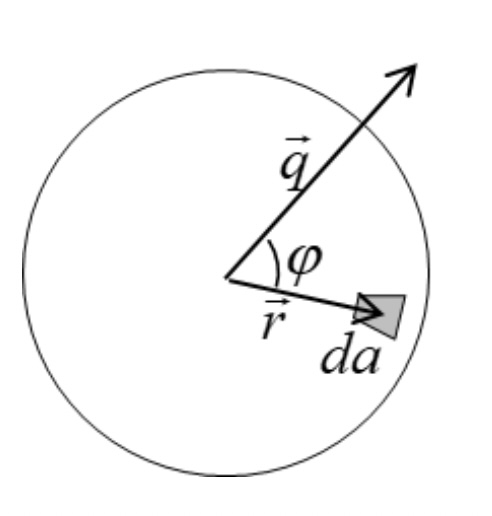
\includegraphics{figs/schema-vett-trasferito-2}
	%    \caption{Sezione d'urto differenziale di una sfera rigida.}
	\label{fig:vett-trasferito2}
\end{marginfigure}

il vettore \(\bm{r}\), che identifica i punti del disco circolare (per
comodità lasciamo cadere l'accento), giace sul piano del bersaglio
\(xy\) a formare un angolo \(\varphi\) con \(\bm{q}\) per cui si ha
\(\bm{q} \cdot \bm{r} = qr \cos \varphi\),ed infine-- adottatele
coordinate cilindriche -- l'elemento d'area vale
\(da = r d \varphi dr\).
Ricordando l'\textbf{ampiezza di diffusione}
\[
	f(\bm{q}) = \frac{ik}{2 \pi} \iint_{S_B} \Gamma(\bm{r}')e^{-i \bm{q} \cdot \bm{r}} \, da
\]
questa si scriverà come
\begin{align*}
	f(\bm{q}) & = \frac{ik}{2 \pi} \int_0^{2 \pi} \int_0^{\infty} \Gamma(r) e^{-iq \cos \varphi r} r \,d \varphi dr                      \\
	& = \frac{ik}{2 \pi} \int_0^R r \left[ \int_0^{2 \pi} e^{-iq \cos \varphi r} d \varphi \right] \, dr                       \\
	& = ik \int_0^R \underbrace{\left[ \frac{1}{2 \pi}\int_0^{2 \pi} e^{-iq \cos \varphi r} d \varphi \right]}_{J_0(qr)} \, dr
\end{align*}
dove \(J_0(qr)\) è nota come \textbf{funzione di Bessel di
ordine zero}:
\[
	J_0(qr) = \frac{1}{2 \pi}\int_0^{2 \pi} e^{-iq \cos \varphi r} d \varphi
\]

\begin{marginfigure}
	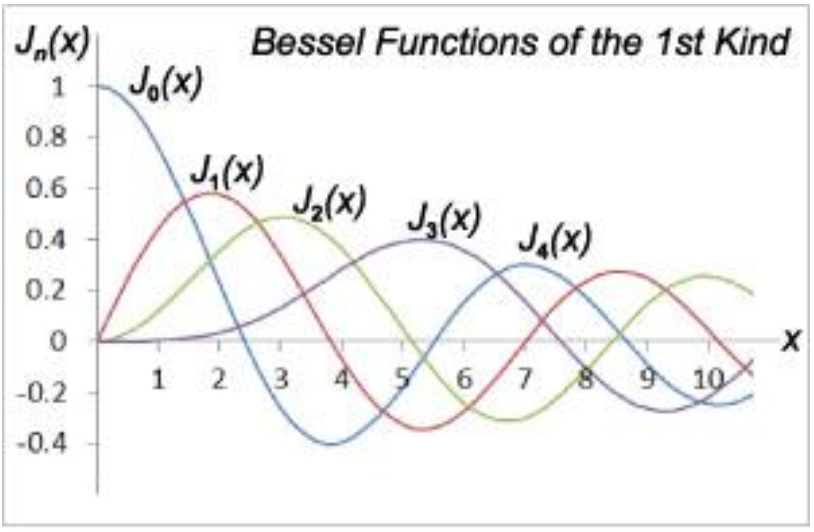
\includegraphics[width = 1.25 \textwidth, height = 1.25 \textheight]{figs/bessel-func-1st-kind}
	\caption{Rappresentazione grafica delle funzioni di Bessel del primo tipo.}
	\label{fig:bessel-func}
\end{marginfigure}

Abbiamo allora la seguente espressione dell'ampiezza di diffusione:
\[
	f(\bm{q}) = ik \int_0^R r J_0(qr) \, dr
\] che può essere integrata per ottenere (Vedi Appendice)
\[
	f(\bm{q}) = ik \frac{R}{q} J_1(qR)
\]
dove \(J_1(qR)\) è la funzione di Bessel di ordine \(1\).
Tenendo ora conto che \(q = k \sin \vartheta\) otteniamo infine
\begin{equation}
	f(\bm{q}) = i \frac{R}{\sin \vartheta} J_1(kR \sin \vartheta)
\end{equation}
Tenendo conto ora della funzione profilo considerata dalla \((25)\) si ottiene la seguente espressione
\[
	\sigma_{diff} = \iint_{S_B} |\Gamma(\bm{r})|^2 \, da = \iint_{S_B} da
\]
dalla quale segue la \textbf{sezione d'urto totale di diffusione del disco assorbente}
\begin{equation}
	\sigma_{diff} = \pi R^2
\end{equation}
Calcoliamo l'ampiezza di diffusione in avanti
\[
	f(\bm{0}) = \frac{ik}{2 \pi} \iint_{S_O} \Gamma (\bm{r}) da = \frac{ik}{2 \pi} \iint_{disco} da = \frac{ik}{2 \pi}
	\pi R^2 = i \frac{kR^2}{2}
\] e ricordando il teorema ottico abbiamo
\[
	\sigma_{tot} = \frac{4 \pi}{k} \Im f(\bm{0}) = \frac{4 \pi}{k} \Im \left(i  \frac{kR^2}{2}\right) = \frac{4 \pi}{k}\frac{kR^2}{2}
\]
da segue la \textbf{sezione dl'urto totale d'interazione del disco assorbente}
\begin{equation}
	\sigma_{tot} = 2 \pi R^2
\end{equation}
Dal teorema ottico infine
\[
	\sigma_{ass} = \sigma_{tot} - \sigma_{diff} = 2\pi ^2 - \pi R^2
\] da cui segue l'espressione della \textbf{sezione d'urto totale di
assorbimento del disco assorbente}
\begin{equation}
	\sigma_{ass} = \pi R^2
\end{equation}

Troviamo allora che la sezione d'urto totale d'interazione di un'onda
piana su di un disco assorbente è il doppio della superficie del disco
stesso, poiché sia la sezione d'urto totale di diffusione che quella di
assorbimento hanno entrambe il valore di quella superficie.
%%%%%%%%%%%%%%%%%%%%%%%%%%%%%%%%%%%%%%%%%%%%%%%%%%%%%%%%%%%%%%%%%%%%%%%%%%%%%%%%%%%%%%%%%%%%%%%%%%%%%%%%%%%%%%%%%%%%%%%%
\section{Il raggio nucleare}\label{sec:raggio-nucleare}
%%%%%%%%%%%%%%%%%%%%%%%%%%%%%%%%%%%%%%%%%%%%%%%%%%%%%%%%%%%%%%%%%%%%%%%%%%%%%%%%%%%%%%%%%%%%%%%%%%%%%%%%%%%%%%%%%%%%%%%%
Nell'ottica, forma, dimensioni ed altre proprietà di un oggetto possono
essere studiate inviando su di esso onde luminose e registrando le onde
emergenti su di uno schermo. Scegliendo la lunghezza d'onda della luce
in modo da avere il potere risolutivo desiderato, sullo schermo apparirà
una figura di diffrazione con una distribuzione dell'intensità luminosa
che caratterizza l'oggetto illuminato. Data l'onda incidente quindi, il
problema sarà quello di risalire dalla distribuzione della intensità
luminosa osservata alle proprietà dell'oggetto illuminato.

In fisica nucleare e subnucleare le cose vanno esattamente nello stesso
modo.

Ciò premesso, i ragionamenti che potrebbero guidare un esperimento per
la \textbf{misura delle dimensioni del nucleo atomico} sono i seguenti:
\begin{enumerate}
	\tightlist
	\item
	\emph{Scelta delle particelle del fascio}. L'uso di fasci di elettroni
	permetterebbe di ottenere dati molto precisi sia per la qualità dei
	fasci disponibili che per la puntiformità delle particelle e
	l'eccellente conoscenza teorica della interazione elettromagnetica. E'
	però chiaro che gli elettroni restituirebbero una `radiografia' della
	distribuzione nucleare dei soli protoni. Volendo ottenere informazioni
	sulla distribuzione di tutti i nucleoni sarebbe meglio utilizzare
	fasci di \emph{neutroni} i quali - interagendo solo fortemente -
	`vedrebbero' sia i protoni che i neutroni senza il `disturbo'
	addizionale della interazione elettromagnetica che invece si avrebbe
	usando fasci di \emph{protoni}. Tali vantaggi competono però con la
	qualità inevitabilmente inferiore dei fasci di neutroni;
	\item
	\emph{Scelta della energia del fascio}. La scelta della energia è
	essenzialmente dettata dal potere risolutivo che si vuole avere nello
	studio della struttura del nucleo per cui la lunghezza d'onda di De
	Broglie delle particelle del fascio deve essere almeno dell'ordine di
	grandezza delle dimensioni nucleari. Nel caso dei neutroni, si avrebbe
	una risoluzione dell'ordine di \(10 \  fm \,(1 fm=10^{-15} m)\) con
	circa \(10 Mev\) di energia cinetica
	\[ \lambda \simeq 10 fm \simeq 10 \frac{1}{200} \frac{\hbar r c}{MeV} \simeq \frac{1}{20} \frac{\hbar  c}{MeV}\]
	\[ E_{cin} = \sqrt{ p^{2}c^{2}+m^{2}c^4 } - mc^{2} \simeq mc^{2} \left(1 + \frac{1}{2} \frac{{p^{2}c^{2}}}{m^{2}c^4}- mc^{2}\right) \simeq \frac{p^{2}}{2m} \simeq \frac{\hbar^{2}k^{2}}{2m}\]
	\[ \simeq 2\pi^{2} \frac{\hbar c^{2}}{mc^{2}\lambda^{2}} \simeq 20 \frac{\hbar^{2} c^{2} }{1000MeV_{1}} \frac{1}{400} \frac{\hbar^{2} c^{2}}{MeV^2} \simeq 8 MeV\]
	\item
	\emph{Processi in gioco}. Difficilmente un sperimento può prescindere
	da una qualche ipotesi/conoscenza dei processi che avranno luogo nelle
	condizioni scelte. Assumendo che i neutroni da \(10 \ MeV\) non
	riescano a trapassare il nucleo atomico, questo potrà essere
	assimilato ad un disco assorbente.
\end{enumerate}

Sulla base di queste considerazioni si potrà costruire un esperimento
per determinare il raggio nucleare, attarverso la misura delle sezioni
d'urto totali e di difusione di neutroni su bersagli materiali.
Ipotizzando che il nucleo possa essere descritto da un disco assorbente
si ha la seguente espressione della sezione d'urto totale (\(28\))
\[
	\sigma = 2 \pi R^2
\]
Si possono allora determinare i raggi nucleari misurando la sezione
d'urto totale di neutroni di circa 10 MeV su bersagli materiali puri
contenenti i diversi tipi di nucleo.

Nella figura è mostrato un grafico della \textbf{sezione d'urto totale e
di assorbimento} di neutroni da 14 MeV in funzione della radice cubica
del numero di nucleoni A del nucleo.
\begin{marginfigure}
	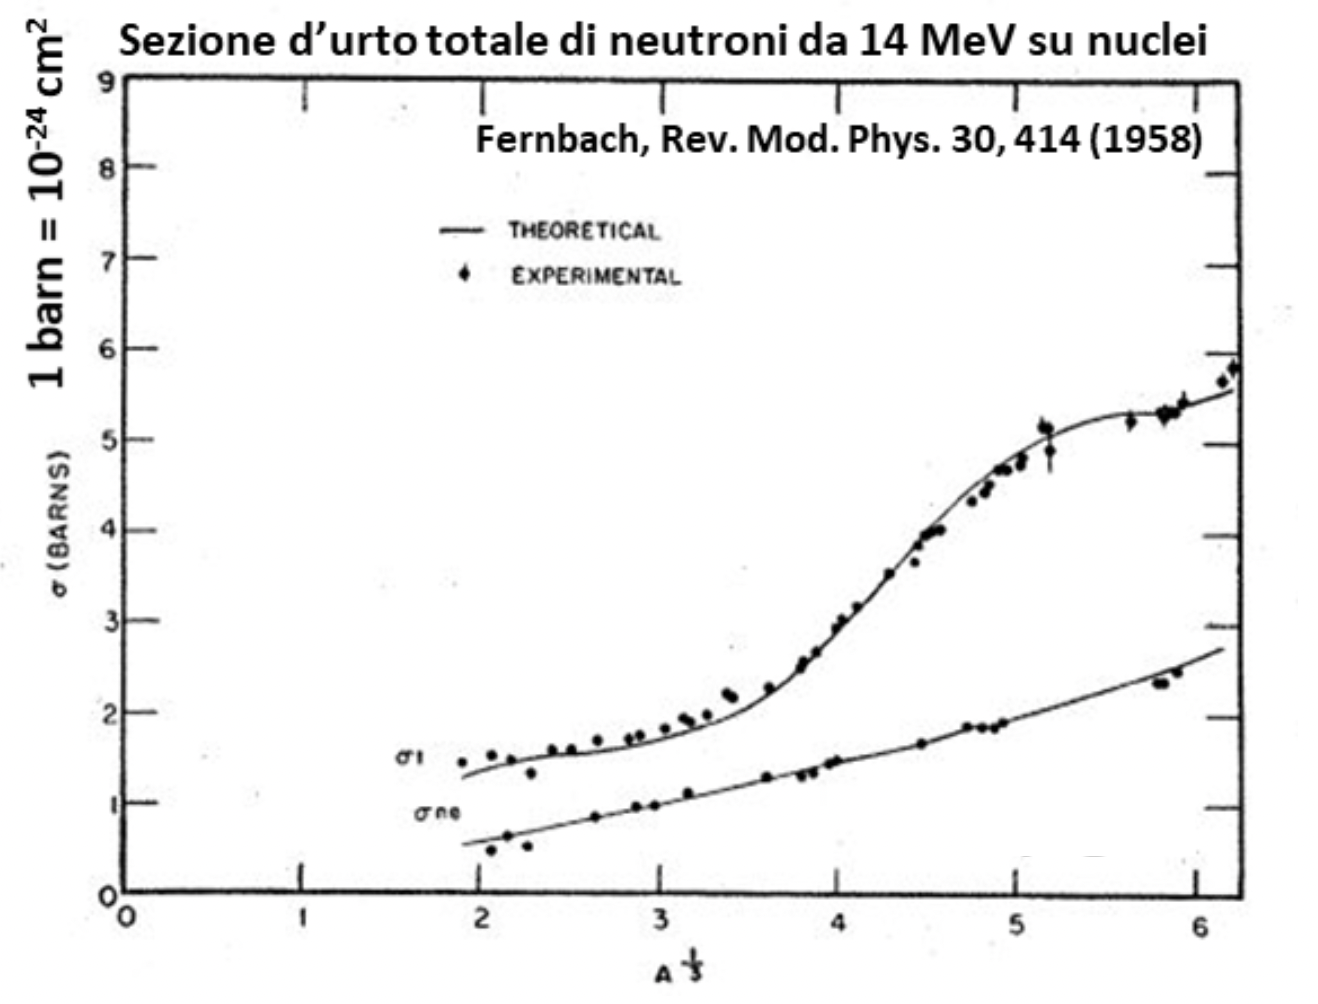
\includegraphics[width = 1.35 \textwidth, height = 1.35 \textheight]{figs/grafico-cross-sect-neutroni}
	%    \caption{Sezione d'urto differenziale di una sfera rigida.}
	\label{fig:cross-section-neutroni}
\end{marginfigure}

Ci serve un modello capace di fornire una relazione tra la sezione d'urto totale ed il numero di nucleoni del nucleo.
Per cominciare, potremmo modellare il nucleo come un \textbf{aggregato sferico di nucleoni} a loro volta assimilati a piccole sfere.
Ipotizzando che la forza che lega netroni e protoni sia a \textbf{corto raggio} con raggio d'azione dell'ordine delle dimensioni del singolo nucleone, il nucleo tenderà ad avere una \textbf{densità volumetrica uniforme} per cui potremo scrivere le seguenti relazioni \[
	V_{Nuc} \simeq \frac{4}{3} \pi R^3 \qquad V_{Nuc} \simeq A\frac{4}{3} \pi {r_{0}}^3
\] dalle quali si ottiene la seguente relazione tra raggio nucleare e numero atomico \[
	R \simeq r_{0} A^{1/3}
\] Immaginando ora il nucleo come un disco assorbente, possiamo sostituire questa relazione nella ($28$) ed ottenere la seguente formula con la quale interpretare i dati \[
	\sigma = 2 \pi r_{0}^{2}(A^{1/3})^{2}
\] In prima approssimazione la formula funziona.
Si noti infatti che i dati hanno effettivamente un andamento ad arco di parabola nella variabile $A^{1/3}$ ma, contrariamente alla previsione della formula, intersecano l'asse verticale ($A=0$) ad un valore di sezione d'urto non nullo.
Ciò significa che dobbiamo aggiungere un termine costante alla sezione d'urto di cui sopra ottenibile solo con l'aggiunta di un termine costante nella espressione del raggio nucleare \[
	R_{Nuc} = r_{0} A^{1/3} + b
\] Bethe suggerì che tale termine dovesse interpretarsi come un una specie di \textbf{'alone nucleare'(nuclear skin), di spessore costante ed uguale per tutti nuclei, dovuto al raggio finito della interazione forte tra nucleoni.} Stimando in circa $0.5 \ barn$ il valore approssimativo della sezione d'urto totale ad $A=0$ possiamo estrarre la corrispondente stima di $b$ \[
	\sigma = 2 \pi R^{2} = 2 \pi (r_{0} A^{1/3} +b)^{2} \quad \sigma(A^{1/3}=0) = 2\pi b^{2} \qquad b = \sqrt{ \frac{\sigma(A^{1/3}=0)}{2 \pi} }\sim 2.8 \ fm
\] Il valore meglio compatibile con i dati sperimentali oggi disponibili è circa $b=2.4 \, fm$.
Una volta determinata la 'skin' nucleare possiamo determinare anche il raggio del nucleone $r_0$.
Leggendo il valore della sezione d'urto totale d'interazione corrispondente ad un secondo nucleo (ad esempio $A^{1/3}=4$ dove $\sigma = 2.8 barn$) possiamo ottenere la seguente stima di $\bm{r_0}$ \begin{gather*}
	\sigma = 2 \pi R^2 = 2 \pi (r_0 A^{1/3} +b)^2  \qquad r_0 = \frac{1}{A^{1/3}} \left( \sqrt{\frac{\sigma}{2 \pi}}-b \right)\\
	r_0 \simeq \frac{1}{4} \left( \sqrt{\frac{2.8 \times 10^{-24}}{2 \pi} } - 2.4 \times 10^{-13} \right) \simeq1.1 \ fm\\
\end{gather*} Informazioni più dettagliate sulla geometria del nucleo possono essere ottenute da esperimenti capaci di misura- re la sezione d'urto differenziale di diffusione.
Modellando il nucleo come un disco circolare assorbente la una sezione d'urto differenziale di diffusione sarà data dalla espressione \[
	\frac{d\sigma_{diff}}{d \Omega} = \frac{R^{2}}{\sin ^{2}\theta}J_{1}^{2}\left( \frac{2 \pi R}{\lambda} \sin \theta \right)
\] che va confrontata con i dati sperimentali mostrati a fianco.
Si nota subito che i dati mostrano un andamento con l'angolo $\theta$ di tipo diffrattivo, in prima approssimazione compatibile con quello di una funzione di Bessel del primo ordine.

È interessante considerare la sezione d'urto differenziale in avanti, ovvero per $\theta$ prossimo a zero.
Sviluppando asintoticamente la funzione di Bessel per piccoli valori dell'argomento si ha \[
	J_{1}(z) \sim \frac{1}{2}z - \frac{1}{16}z^{3}
\] da cui - sostituendo - otteniamo la \textbf{sezione d'urto differenziale di diffusione in avanti} dalla quale si può ottenere una nuova \textbf{stima del raggio nucleare}
\[
	\frac{d\sigma_{diff}}{d \Omega} = \frac{R^{2}}{\sin ^{2}\theta}J_{1}^{2}\left( \frac{2 \pi R}{\lambda} \sin \theta \right) \sim \frac{R^{2}}{\sin ^{2}\theta} \frac{1}{4} \frac{4 \pi^{2} R^{2}}{\lambda^{2}} \sin ^{2} \theta \sim \frac{\pi^{2}R^{4}}{\lambda^{2}}
\]
\begin{marginfigure}
	\centering
	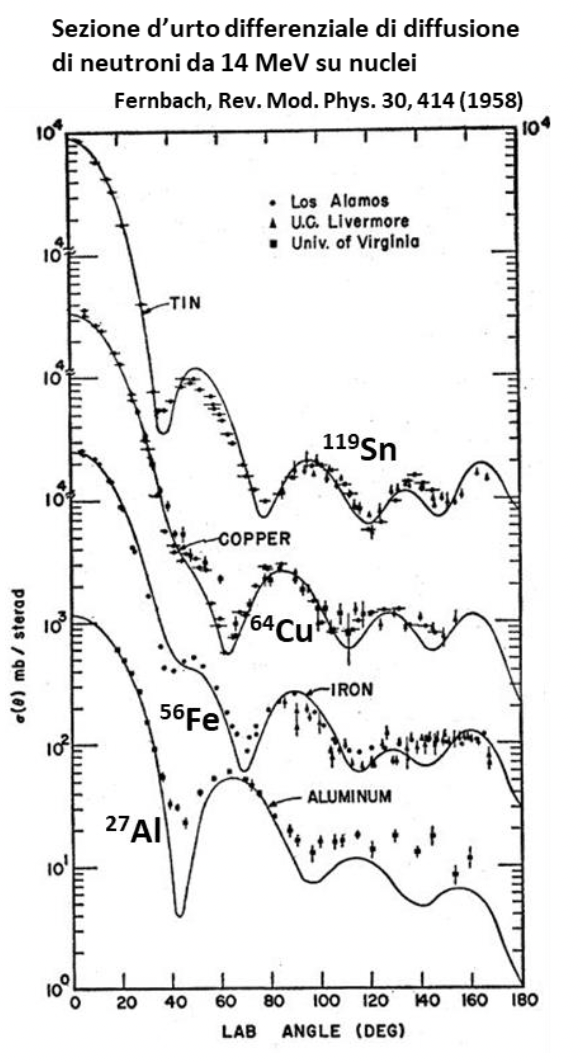
\includegraphics[width = 1.25 \textwidth,height = 1.25 \textheight]{figs/grafico-cross-sect-neutroni-2}
	%    \caption{Sezione d'urto differenziale di una sfera rigida.}
	\label{fig:cross-section-neutroni2}
\end{marginfigure}
Dalla figura si vede chiaramente che tale sezione d'urto a $\theta=0$ aumenta rapidamente con il numero di nucleoni $A$.

na seconda possibilità consiste nel lavorare sui minimi di diffrazione la cui spaziatura -- come noto dall'ottica -- deve dipendere dal raggio del disco ovvero dal raggio nucleare.

Ora è noto che le funzioni di Bessel si annullano ripetutamente, un fatto che però non trova corrispondenza nell'andamento delle sezioni d'urto di diffuzione misurate che, pur avendo dei minimi pronunciati, non si annullano mai.
Questo fatto indica che modellizzare il nucleo come un disco completamente assorbente non è del tutto appropriato e che esiste un certo grado di trasparenza del nucleo rispetto ai neutroni incidenti.
Trascurando per ora questo fatto ed assumendo che i minimi della sezione d'urto corrispondano agli zeri della funzione di Bessel, abbiamo nel caso del primo zero \[
	J_{1}\left( \frac{2 \pi R}{\lambda}\sin \theta = 3.832 \right)
\] da cui si ottiene la seguente espressione \[
	R = \frac{3.832}{2 \pi} \frac{\lambda}{\sin \theta}
\] che fornisce un'altra stima del raggio nucleare a partire dalla posizione angolare del primo minimo della sezione d'urto differenziale di diffusione.

Per estrarne in modo corretto tutto il contenuto informativo, sarebbe necessario eseguire un 'fit' utilizzando il corrispondente chi-quadrato come criterio di bontà e affidabilità della funzione teorica adottata.
In questo modo otterremmo un solo valore del raggio nucleare piuttosto che i due stimati e, soprattutto, verificheremmo che l'ipotesi che il nucleo assorba totalmente i neutroni incidenti è troppo drastica poiché non riesce a riprodurre correttamente l'andamento delle sezioni d'urto di diffusione.

I dati richiedono l'ipotesi che il nucleo sia parzialmente trasmittente.
Si è pensato quindi di modellizzare il nucleo per mezzo di un potenziale complesso dando origine al cosiddetto modello ottico del nucleo(la parte reale del potenziale è solitamente assunta nella forma di Saxon-Woods mentre quella immaginaria nella forma di una gaussiana).
%%%%%%%%%%%%%%%%%%%%%%%%%%%%%%%%%%%%%%%%%%%%%%%%%%%%%%%%%%%%%%%%%%%%%%%%%%%%%%%%%%%%%%%%%%%%%%%%%%%%%%%%%%%%%%%%%%%%%%%%
\section{Energia di legame nucleare}\label{sec:energia-di-legame-nucleare}
%%%%%%%%%%%%%%%%%%%%%%%%%%%%%%%%%%%%%%%%%%%%%%%%%%%%%%%%%%%%%%%%%%%%%%%%%%%%%%%%%%%%%%%%%%%%%%%%%%%%%%%%%%%%%%%%%%%%%%%%


Si immagini un sistema formato da due sferette omogenee di massa m e raggio $R$, soggette alla mutua attrazione gravitazionale, disposte in quiete l'una accanto all'altra con una energia potenziale iniziale $E_{i}$.
Sappiamo che per separare le sferette dobbiamo applicare su una di esse una forza esterna uguale e contraria a quella attrattiva in modo da portarla all'infinito (avendo avuto cura di fissare l'altra!).
Nel linguaggio della meccanica dobbiamo compiere lavoro contro la forza attrattiva gravitazionale che tiene unite le sferette, nel più generale linguaggio della energia dobbiamo fornire energia al sistema legato in modo da separarlo nei suoi componenti portandolo ad una energia potenziale finale che indicheremo con $E_{f}$ (in questo caso nulla).
Tale energia viene detta energia di legame del sistema e soddisfa la seguente relazione

\begin{marginfigure}
	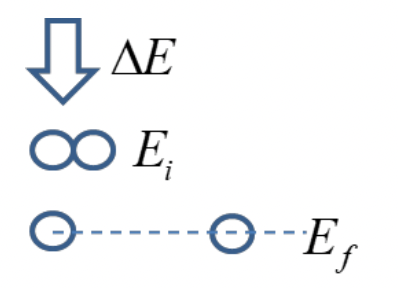
\includegraphics{figs/en-legame}
	%    \caption{Sezione d'urto differenziale di una sfera rigida.}
	\label{fig:en-legame}
\end{marginfigure}

\begin{equation}
	\Delta E = E_{i} = E_{f}
\end{equation}
Ora immaginiamo di volerla determinare.
In linea di principio potremmo utilizzare \textbf{tre diversi metodi}:
\begin{enumerate}
	\def\labelenumi{\arabic{enumi}.}
	\tightlist
	\item
	disponendo di una espressione esplicita della forza, potremmo
	calcolarla teoricamente \[
								\Delta E = \int_{2 R}^{\infty} \bm{F}_{est} \cdot d\bm{l} = \int_{2 R}^{\infty} G \frac{m^{2}}{r^{2}} \, dr
								= G \frac{m^{2}}{2R}
	\]
	\item
	non disponendo della espressione teorica potremmo misurare
	ripetutamente la forza applicata sulla sferetta e sommare in modo da
	ottenere il lavoro compiuto \[
									\Delta E = \int _{2R}^{\infty} \bm{F}_{est} \cdot d\bm{l}
	\]
	\item
	non disponendo della espressione teorica potremmo anche affidarci alla
	teoria della relatività ristretta (TRR). Sappiamo infatti che ad ogni
	forma di energia \(E\)corrisponde una massa inerziale equivalente
	\(M\) data dalla ben nota equazione \(M=E/c^{2}\). Su questa base,
	dato che il contenuto energetico del sistema iniziale legato e del
	sistema finale separato sono diversi, dobbiamo aspettarci che diverse
	siano pure le corrispondenti masse inerziali. In particolare da
	\(\Delta E = E_{i} = E_{f}\) otteniamo \(E_{f} > E_{i}\) (poiché
	\(\Delta E >0\)) da cui discende pure che \(M_{f} > M_{i}\) . Dalle
	espressioni relativistiche \[
								   E_{f} = M_{f}c^{2} \qquad E_{i} = M_{i}c^{2}
	\]otteniamo allora la seguente differenza di massa detta
	\textbf{difetto di massa del sistema legato} \[
													 (M_{f}-M_{i}) = \frac{\Delta E}{c^{2}}
	\] la quale offre una terza via per accedere all'energia di legame.
\end{enumerate}

\begin{marginfigure}
	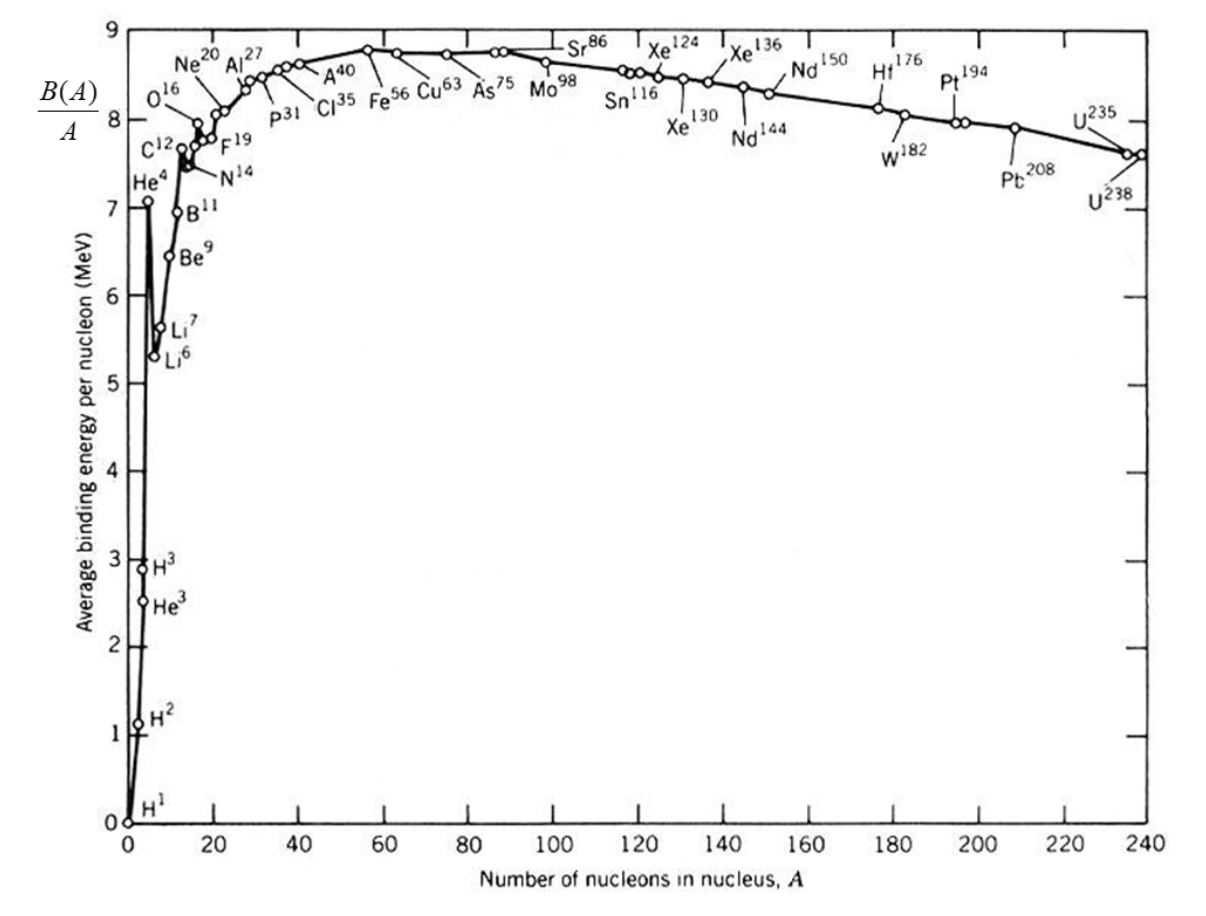
\includegraphics[width = 1.3 \textwidth,scale = 1]{figs/en-legame-graph}
	\caption{Grafico dell'energia di legame media per nucleone in funzione del numero di nucleoni $A$.}
	\label{fig:en-legame-graph}
\end{marginfigure}

Nel caso di un sistema macroscopico di due masse legate dalla forza
gravitazionale, il metodo \(1\) risulta praticabile poiché conosciamo
l'espressione teorica della forza. Superando un certo numero di
difficoltà sperimentali potremmo anche utilizzare il metodo \(2.\)
Certamente nessun fisico sperimentale sarebbe però in grado di
utilizzare il metodo \(3\) dato che dovrebbe misurare il seguente
difetto di massa \[
					 (M_{f}-M_{i}) = \frac{\Delta E}{c^{2}} = G \frac{m^{2}}{2Rc^{2}} = 5.6 \times 10^{-54} MeV
\] Nel caso della interazione forte tra nucleoni le cose vanno
diversamente. Il metodo \(1\) richiederebbe una conoscenza della forte
che non abbiamo poiché -- appunto -- dobbiamo ancora determinarne le
proprietà. Il metodo \(2\) è chiaramente inapplicabile ad un sistema
microscopico. Il metodo \(3\), basato sulla TRR, potrebbe essere
applicabile qualora il difetto di massa del sistema fosse consistente.
Ora i dati sperimentali mostrano che \textbf{l'energia potenziale
dell'interazione attrattiva tra nucleoni è tale da fornire un
apprezzabile contributo negativo alla inerzia del nucleo}, generando una
differenza misurabile tra la massa dei nucleoni componenti e quella del
nucleo stesso.

Sulla base di quanto detto, siamo ora in grado di fornire la seguente
\textbf{definizione operativa della energia di legame} ovvero della
\emph{energia necessaria per separare il nucleo nei nucleoni componenti}

\begin{equation}
	B\left( {}^{A}_{Z}X \right)  = \left[ Nm_{n} + Zm_{p} -m_{N}\left( {}^{A}_{Z}X \right) \right]c^{2}
\end{equation}
dove $m_{n},m_{p},m_{N}$ sono rispettivamente le masse del neutrone, del protone e del nucleo
\sidenote{Vale la pena precisare che le masse nucleari sono misurabili con minore precisione di quelle atomiche per cui è utile ricavare le prime delle seconde attraverso la relazione \[
	m_{A}\left( {}^{A}_{Z}X \right) = m_{N}\left( {}^{A}_{Z}X \right)+Zm_{e} - \frac{1}{c^{2}}\sum_{i = 1}^{Z}B_{i}^{el}
\] dove $m_{A}$ è la massa dell'atomo corrispondendente al nucleo in esame.}.
Limitando la rappresentazione ai soli nuclidi stabili (nel caso vi fosse più di un isotopo stabile si sceglie quello più abbondante) si ottiene l'energia di legame media per nucleone $B/A$ in funzione di $A$ mostrata qui a fianco.

Il quoziente $B/A$ dà una indicazione quantitativa del grado di stabilità del nuclide e permette di stabilire se una data reazione nucleare sia esoenergetica o endoenergetica e, dunque, se possa avvenire spontaneamente oppure no.

Dal grafico in figura \ref{fig:en-legame-graph} possiamo trarre alcune conclusioni generali:
\begin{enumerate}
	\item Ci sono configurazioni nucleari particolarmente stabili quali ${}^{4}He, {}^{12}_{}C, {}^{16}_{}O, \dots$
	\item a parte queste eccezioni, l'energia di legame media per nucleone ha un andamento regolare.
	      Aumenta rapidamente con il numero di nucleoni fino ad un valore dell'ordine degli $8 \ MeV$ per poi diminuire assai lentamente
	\item i nucleo piu stabili sono ${}^{56}_{}Fe$ e ${}^{62}_{}Ni$.
	      Ciò significa che i nuclei pesanti alla sua destra pososno raggiungere configurazioni piu stabili (ovvero con $B / A$ piu elevato) aumentando $A$, ovvero aggregandosi in nuclei piu grandi.
	      Detto in altri termini ciò significa che \textbf{le reazioni di fissione dei nuclei pesanti e e quelle di fusione dei nuclei leggeri sono esoenergetiche} ovvero producono energia qualora si sia in grado di innescarle;
	\item dal punto precedente consegue che \textbf{le reazioni di fusione dei nuclei leggeri e fissione dei nuclei pesanti} costituiscono la doppia opportunità offerta dalla fisica nucleare per la produzione di energia.

\end{enumerate}

La via della fusione nucleare è stata scelta dalle stelle. Oggi sappiamo
che una stella come il sole ricava la quasi totalità della energia
(circa il \(98 \%\)) dalla fusione di nuclei d'idrogeno in nuclei di
elio.
L'energia prodotta dalle reazioni di fusione fluisce verso
l'esterno.
Tale flusso, nella forma di energia cinetica dei prodotti
delle reazioni di fusione, fornisce la spinta verso l'esterno capace di
opporsi alla contrazione gravitazionale mantenendo il sole in una
situazione di equilibrio di forze detto equilibrio idrostatico.

Dal grafico si può leggere il decorso del processo una volta esaurito
l'idrogeno: la contrazione gravitazionale prenderà il sopravvento
comprimendo la materia fino al punto da innescare le reazioni di fusione
di tre nuclei di elio in un nucleo di carbonio stabilendo un nuovo
periodo di equilibrio.
Le fasi di equilibrio e contrazione si
alterneranno fino alla fusione del silicio in ferro quando la
contrazione gravitazionale - non potendo innescare altre reazioni di
fusione - procederà inarrestabile facendo collassare la stella che
espellerà in modo esplosivo gli strati più esterni lasciando un residuo
compatto di materia in uno stato degenere.

La via della \emph{fissione nucleare} trova invece una sua applicazione
nei reattori nucleari.